% !TEX program = xelatex
% 本周（2026-10-19 至 2026-10-25）Daily Exercise List 回顾 · 30 题详解版
% 自包含单文件：导言区 + 封面/概览/议程 + 两部分逐题详解 + 答案速查/方法卡/易错点/自测
% 编译：xelatex 跑三遍（页码 \pageref 需要两遍以上；中文字体 Microsoft YaHei）
\documentclass[aspectratio=169,10pt,fontset=none]{ctexbeamer}

% ---------- 中英文字体 ----------
\usepackage{fontspec}
\setCJKmainfont{Microsoft YaHei}
\setCJKsansfont{Microsoft YaHei}

% ---------- 数学与图形 ----------
\usepackage{amsmath,amssymb}
\usepackage{booktabs}
\usepackage{array}
\usepackage{colortbl}
\usepackage{graphicx}
\graphicspath{{./}{Attachments/}{../Attachments/}{../../Attachments/}}
\usepackage{tikz}
\usetikzlibrary{arrows.meta,positioning,calc}

% ---------- 配色（沿用库内讲义配色） ----------
\definecolor{ink}{HTML}{1F3864}
\definecolor{accent}{HTML}{C00000}
\definecolor{gold}{HTML}{BF8F00}
\definecolor{greenink}{HTML}{2E6B2E}
\definecolor{paper}{HTML}{F5F7FA}

\usetheme{default}
\usecolortheme[named=ink]{structure}
\setbeamertemplate{navigation symbols}{}
\setbeamertemplate{itemize items}[circle]
\setbeamercolor{structure}{fg=ink}
\setbeamercolor{frametitle}{fg=ink}
\setbeamercolor{block title}{bg=ink!12,fg=ink}
\setbeamercolor{block body}{bg=ink!4,fg=black}
\setbeamercolor{block title alerted}{bg=accent!12,fg=accent}
\setbeamercolor{block body alerted}{bg=accent!4,fg=black}
\setbeamercolor{block title example}{bg=greenink!14,fg=greenink}
\setbeamercolor{block body example}{bg=greenink!5,fg=black}
\setbeamerfont{frametitle}{size=\large,series=\bfseries}
\setbeamerfont{footline}{size=\scriptsize}
\setbeamertemplate{frametitle}{\vskip3pt\insertframetitle\par\vskip1.5pt%
  \textcolor{accent}{\rule{\textwidth}{0.7pt}}\vskip-3pt}
\setbeamertemplate{footline}{%
  \hbox to \paperwidth{\hspace{8pt}%
    \textcolor{ink!55}{本周 Daily Exercise 回顾\ \ ·\ \ 10-19 -- 10-25\ \ ·\ \ 30 题详解版}\hfill
    \textcolor{ink!55}{\insertframenumber\,/\,\inserttotalframenumber}\hspace{9pt}}\vskip5pt}
\setbeamersize{text margin left=0.75cm,text margin right=0.75cm}
\setlength{\parindent}{0pt}
\setlength{\parskip}{2pt}
\AtBeginDocument{%
  \setlength{\abovedisplayskip}{3pt}\setlength{\belowdisplayskip}{3pt}%
  \setlength{\abovedisplayshortskip}{2pt}\setlength{\belowdisplayshortskip}{2pt}}

% 题号标记
\newcommand{\ex}[1]{\textcolor{accent}{\footnotesize\bfseries #1}}
\newcommand{\key}[1]{\textcolor{ink}{\bfseries #1}}
\newcommand{\starpt}{\textcolor{accent}{\bfseries$\ast$}}

\hypersetup{pdftitle={本周 Daily Exercise 回顾（2026-10-19 至 10-25，30 题详解版）},
  pdfsubject={Artin Algebra 2e, Ch. 6 and Ch. 7 Sections 5--7: 30 exercises weekly review},
  pdfauthor={exercise\_abstract}}
\title{本周 Daily Exercise 回顾（2026-10-19 至 10-25，30 题详解版）}
\author{exercise\_abstract}

\begin{document}
% ============================================================ 1 标题页
\begin{frame}[plain]
  \begin{tikzpicture}[remember picture,overlay]
    \fill[ink] (current page.north west) rectangle ([yshift=-4.75cm]current page.north east);
    \node[anchor=north west,text=white,font=\fontsize{25}{29}\selectfont\bfseries]
      at ([xshift=1.0cm,yshift=-0.92cm]current page.north west) {本周 Daily Exercise 回顾};
    \node[anchor=north west,text=white!90]
      at ([xshift=1.02cm,yshift=-2.08cm]current page.north west)
      {\large 覆盖 2026-10-19 -- 10-25（5 份清单，30 题）\quad·\quad 逐题详解版};
    \node[anchor=north west,text=white!75]
      at ([xshift=1.02cm,yshift=-2.86cm]current page.north west)
      {\normalsize Artin \textit{Algebra} 2e, Ch.~6 + Ch.~7 \S5--\S7\quad·\quad 群论 24 + 线性代数 6\quad·\quad 难度 5 / 8 / 17};
    \node[anchor=north east,text=white!60,font=\small]
      at ([xshift=-1.0cm,yshift=-0.92cm]current page.north east) {exercise\_abstract};
    \node[anchor=west,text=white!55,font=\tiny]
      at ([xshift=1.02cm,yshift=-4.45cm]current page.north west)
      {数据来源：\texttt{10 - Daily Exercise Lists} 的五份清单；题面与来源取自 30 篇习题笔记，数学结论经复核（G225 的计数已修正）；快照 2026-10-25 19:16};
  \end{tikzpicture}
  \vspace*{4.9cm}
  \begin{columns}[T,onlytextwidth]
    \begin{column}{0.50\textwidth}
      \begin{block}{两条主线（本周清单的两区）}
        \scriptsize
        \begin{itemize}\setlength{\itemsep}{1pt}
          \item \key{Random Review（15 题，Artin Ch.~6）}\\
                平面等距群、壁纸群、多面体对称、群作用、矩阵/格的作用
          \item \key{Systematic Progress（15 题，Artin Ch.~7 \S5--\S7）}\\
                $S_n$ 类方程与 $A_n$ 分裂、$p$-群、正规化子、Sylow
        \end{itemize}
      \end{block}
    \end{column}
    \begin{column}{0.47\textwidth}
      \begin{block}{这一版的用法与边界}
        \scriptsize
        \begin{itemize}\setlength{\itemsep}{1pt}
          \item 每题：完整题面 → 一句思路 → \textbf{显示中间式的推导} → 具体验算/反例
          \item 5 份清单中 10-21、10-22 没有题单；讲义按“有题单的 5 天”统计
          \item 这是\textbf{快照}：10-25 题单 19:15 才生成；Random Review 仍可能追加
          \item 第 \pageref{sec:answers} 页起是 30 题速查表、方法卡、易错点与自测
        \end{itemize}
      \end{block}
    \end{column}
  \end{columns}
\end{frame}

% ============================================================ 2 本周概览
\begin{frame}[t]{一、本周概览：5 份题单、30 题、两个独立队列}
  \label{sec:overview}
  \centering
  \scriptsize
  \setlength{\tabcolsep}{3pt}
  \renewcommand{\arraystretch}{1.14}
  \begin{tabular}{@{}l l l@{}}
    \toprule
    日期 & Random Review（3 题） & Systematic Progress（3 题）\\
    \midrule
    10-19（一） & G192，G149，G166 & G215，G216，G217\\
    10-20（二） & G157，G181，G173 & G218，G219，LA304\\
    \rowcolor{ink!7} 10-21（三） & \multicolumn{2}{c}{无题单（当天未生成；不补抽）}\\
    \rowcolor{ink!7} 10-22（四） & \multicolumn{2}{c}{无题单（当天未生成；不补抽）}\\
    10-23（五） & G153，G175，G170 & LA305，LA306，G220\\
    10-24（六） & G109，LA298，G16 & G221，G222，G223\\
    10-25（日） & G151，LA300，LA192 & G224，G225，G226\\
    \midrule
    合计 & \textbf{15} 题（Ch.~6） & \textbf{15} 题（Ch.~7 \S5--\S7）\\
    \bottomrule
  \end{tabular}
  \vspace{0.35em}
  \raggedright
  \begin{columns}[T,onlytextwidth]
    \begin{column}{0.49\textwidth}
      \begin{exampleblock}{\footnotesize 数据观察}
        \scriptsize
        \begin{itemize}\setlength{\itemsep}{1pt}
          \item \textbf{Random Review 本周 15 题}：全部来自 Artin Ch.~6（几何、壁纸群、多面体、群作用、矩阵/格），与上周 Random 为 0 不同。
          \item \textbf{10-21、10-22 无题单}：不补抽、不臆造；讲义只覆盖实际生成的 5 天。
          \item 30 题全部互不重复；Systematic 按原书题号推进 \S5.8 $\to$ \S7.4。
        \end{itemize}
      \end{exampleblock}
    \end{column}
    \begin{column}{0.49\textwidth}
      \begin{block}{\footnotesize 难度、来源与快照}
        \scriptsize
        入门 5 · 中等 8 · 高级 17。\\[1pt]
        Artin 2e Ch.~6（M.6, 1.1, 5.3--5.5, 6.2--6.6, 7.4, 7.9, 8.1, 9.3, 10.1, 11.1, 11.3, 12.1）与 Ch.~7 \S5--\S7，印刷 pp.~188--194 / 223--224，PDF pp.~200--206 / 235--236；\ex{G220}、\ex{G222}、\ex{G224} 另含 Lang I.16/I.20/I.21。\\[1pt]
        \starpt 快照：2026-10-25 19:16（10-25 题单 19:15 生成）；题单之后若追加，以库内文件为准。
      \end{block}
    \end{column}
  \end{columns}
\end{frame}

% ============================================================ 3 议程
\begin{frame}[t]{二、怎么用：110 分钟议程与三种用法}
  \label{sec:agenda}
  \begin{columns}[T,onlytextwidth]
    \begin{column}{0.54\textwidth}
      \centering
      \scriptsize
      \setlength{\tabcolsep}{3pt}
      \renewcommand{\arraystretch}{1.2}
      \begin{tabular}{@{}l l r@{}}
        \toprule
        时间 & 内容 & 起始页\\
        \midrule
        10 分钟 & 框架：Ch.~6 与 Ch.~7 两条工具线 & \pageref{sec:framework1}\\
        45 分钟 & Random Review 15 题：等距群/壁纸群/多面体/作用 & \pageref{sec:random}\\
        45 分钟 & Systematic 15 题：$S_n$、$p$-群、正规化子、Sylow & \pageref{sec:sys}\\
        10 分钟 & 速查表、方法卡、易错点、当场自测 & \pageref{sec:answers}\\
        \bottomrule
      \end{tabular}
    \end{column}
    \begin{column}{0.43\textwidth}
      \begin{block}{\footnotesize 三种用法}
        \scriptsize
        \begin{itemize}\setlength{\itemsep}{1pt}
          \item \textbf{通读}：每题“题面 → 思路 → 详解 → 验算”完整走一遍；
          \item \textbf{讲题}：先让学生说该算哪个量，再翻到详解页对照；
          \item \textbf{复习}：只看第 \pageref{sec:answers} 页起的速查表与方法卡，忘了再回跳。
        \end{itemize}
      \end{block}
      \begin{alertblock}{\footnotesize 时间不够时的取舍}
        \scriptsize
        30 题一次讲完偏紧，建议分两次：先 Random（第 \pageref{sec:random} 页起），再 Systematic（第 \pageref{sec:sys} 页起）。若只有 60 分钟，优先 G153、G16、G219、G226 四道长题，其余快速过结论。
      \end{alertblock}
    \end{column}
  \end{columns}
  \vspace{0.2em}
  {\scriptsize\color{ink!70} 页脚给出当前页/总页数；所有页码引用由 \LaTeX{} 标签自动生成，增删页面后重编译即可同步。}
\end{frame}

% ============================================================ 4 框架 1/2
\begin{frame}[t]{三、框架 1/2：Random Review 的工具箱（Artin Ch.~6）}
  \label{sec:framework1}
  \begin{columns}[T,onlytextwidth]
    \begin{column}{0.49\textwidth}
      \begin{block}{\footnotesize 平面等距群与壁纸群}
        \scriptsize
        $M=\{\text{平移}\}\rtimes O(2)$；离散子群 $G$ 有短正合列
        \[ 1\to L\to G\to \overline G\to 1, \]
        $L$ 为平移格，$\overline G\le O(2)$ 为点群。晶体限制：$\overline G=C_n$ 或 $D_n$，$n\in\{1,2,3,4,6\}$。\\[1pt]
        壁纸群按点群计数：$C_1,C_2,C_3,C_4,C_6$ 各 1；$D_1:3$，$D_2:4$，$D_3:2$，$D_4:2$，$D_6:1$，共 \textbf{17}。\\
        \key{本周用点}：G149 的指数、G153 的完整列表、G151 的 $D_1$ 三类、G157 的稳定化子。
      \end{block}
      \begin{block}{\footnotesize 多面体与对偶}
        \scriptsize
        旋转群：$T\cong A_4$（12），$O\cong S_4$（24），$I\cong A_5$（60）；允许反射时乘 $C_2$，阶为 $24,48,120$。\\[1pt]
        对偶（十二面体 $\leftrightarrow$ 二十面体）保持对称群：G181；G166 用“面传递 $\times$ 固定面的 $D_5$”算阶。
      \end{block}
    \end{column}
    \begin{column}{0.49\textwidth}
      \begin{block}{\footnotesize 群作用与轨道}
        \scriptsize
        轨道--稳定化子：$|Gs|=[G:G_s]$。传递作用 $\leftrightarrow$ 陪集作用 $G/H$；核 $=\{g:gs=s\ \forall s\}$ 正规（G175）。\\
        $S_3$ 在 4 点上的作用按轨道分拆分类：$1^4,\ 2+1+1,\ 2+2,\ 3+1$（G173）；$D_3$ 在三元子集上的轨道大小 $2,6,6,6$（G170）。
      \end{block}
      \begin{block}{\footnotesize 矩阵与格的作用}
        \scriptsize
        \begin{itemize}\setlength{\itemsep}{0pt}
          \item 合同作用 $P*A=PAP^{\mathsf T}$：验证作用公理（LA300）；
          \item 双边等价 $(P,Q)*A=PAQ^{-1}$：轨道 $=$ 秩层（LA298）；
          \item 指数 $p$ 子格 $\leftrightarrow$ $\mathbb F_p^2$ 中的直线，共 $p+1$ 个（LA192，$p=3$ 时 4 个）；
          \item 平面图案的对称群：滑移反射 $g$、平移 $t$、半转 $s$ 的关系决定 $\mathbb Z$ 或 $D_\infty$（G16、G109）。
        \end{itemize}
      \end{block}
    \end{column}
  \end{columns}
\end{frame}

% ============================================================ 5 框架 2/2
\begin{frame}[t]{三、框架 2/2：Systematic Progress 的工具箱（Artin Ch.~7 \S5--\S7）}
  \label{sec:framework2}
  \begin{columns}[T,onlytextwidth]
    \begin{column}{0.49\textwidth}
      \begin{block}{\footnotesize $S_n$ 的类方程与 $A_n$ 分裂}
        \scriptsize
        共轭类由轮换型决定；轮换型 $1^{m_1}2^{m_2}\cdots$ 的中心化子
        \[ |Z(\sigma)|=\prod_k k^{m_k}m_k!,\qquad |C(\sigma)|=\frac{n!}{|Z(\sigma)|}. \]
        偶 $S_n$-类在 $A_n$ 中保持一类 $\iff$ 中心化子含奇置换；否则分裂成两个等大类。分裂 $\iff$ 轮换长度全为奇数且互不相同（含 1-轮换）。\\
        \key{本周用点}：G217、G218、G219、G215、G216。
      \end{block}
      \begin{block}{\footnotesize $p$-群与共轭作用}
        \scriptsize
        不动点定理：$|S|\equiv|S^G|\pmod p$；共轭作用给 $|Z(G)|\equiv|G|\pmod p$。\\
        $H<G$ 为有限 $p$-群的真子群 $\Rightarrow N_G(H)>H$，且 $H$ 含于某个指数 $p$ 的正规子群（G221）；最小素因子阶正规子群中心（G220）。
      \end{block}
    \end{column}
    \begin{column}{0.49\textwidth}
      \begin{block}{\footnotesize 正规化子与三角子群}
        \scriptsize
        $B\le GL_n$ 上三角可逆、$U$ 单位上三角：$B=N(U)=N(B)$（LA305）；$B$ 与下三角 $L$ 由 $J$ 共轭（LA304）。\\
        置换矩阵子群：$N(P)=\{P_\sigma(aI+bJ):a\ne0,\ a+nb\ne0\}$，$n=6$ 的外自同构被 trace 排除（LA306）。
      \end{block}
      \begin{block}{\footnotesize Sylow 与单性}
        \scriptsize
        $|G|=p^e m$，$p\nmid m$：Sylow $p$-子群存在、共轭；$n_p\mid m$，$n_p\equiv1\pmod p$。\\
        Sylow 可沿包含 $G_1\subset G_2$ 延拓（G224）；$\binom{p^e m}{p^e}\equiv m\pmod p$（G223，Lucas）。\\
        单性排除：$pq$、$p^2q$ 阶无单群（G226）；正规子群不能覆盖群（G222）；20 阶群中 5 阶元恰有 4 个（$n_5=1$，G225）。
      \end{block}
    \end{column}
  \end{columns}
\end{frame}

% ============================================================ 6 Random 分隔页
\begin{frame}[t]{四、随机复习（Random Review）：15 题，Artin Ch.~6}
  \label{sec:random}
  \begin{block}{\footnotesize 本部分覆盖}
    \scriptsize
    10-19：G192, G149, G166\quad·\quad 10-20：G157, G181, G173\quad·\quad 10-23：G153, G175, G170\\
    10-24：G109, LA298, G16\quad·\quad 10-25：G151, LA300, LA192\\[2pt]
    题目从“平面图案/壁纸群的对称”到“多面体对偶、群作用、矩阵与格的作用”，以几何直观和轨道计数为主。
  \end{block}
  \begin{columns}[T,onlytextwidth]
    \begin{column}{0.49\textwidth}
      \begin{exampleblock}{\footnotesize 读法}
        \scriptsize
        每题先问“这个对称群/作用的点群或轨道是什么”，再算指数、轨道大小或稳定化子；遇到图案题，先看图上有没有旋转中心、镜轴、滑移轴。
      \end{exampleblock}
    \end{column}
    \begin{column}{0.49\textwidth}
      \begin{block}{\footnotesize 本周的 5 张题图}
        \scriptsize
        G157、G153、G109、G16 直接依赖 Artin 原图；讲义从库内已核对的图片资产嵌入，并在题面后给出印刷/PDF 页。
      \end{block}
    \end{column}
  \end{columns}
  \vspace{0.2em}
  {\scriptsize\color{ink!70} 本部分从第 \pageref{ex:G192} 页开始；顺序与题单日期一致。}
\end{frame}

% ============================================================ 7 Systematic 分隔页
\begin{frame}[t]{五、系统推进（Systematic Progress）：15 题，Artin Ch.~7 \S5--\S7}
  \label{sec:sys}
  \begin{block}{\footnotesize 本部分覆盖}
    \scriptsize
    10-19：G215, G216, G217\quad·\quad 10-20：G218, G219, LA304\quad·\quad 10-23：LA305, LA306, G220\\
    10-24：G221, G222, G223\quad·\quad 10-25：G224, G225, G226\\[2pt]
    三条线：$S_n$ 的类方程与 $A_n$ 分裂（5 题）→ 正规化子与三角/置换矩阵（6 题）→ Sylow 与单性（4 题）。
  \end{block}
  \begin{columns}[T,onlytextwidth]
    \begin{column}{0.49\textwidth}
      \begin{exampleblock}{\footnotesize 读法}
        \scriptsize
        每题先定位“用哪个量”：类大小/中心化子、正规化子、$n_p$ 的整除与同余；再写具体类方程或具体子群。
      \end{exampleblock}
    \end{column}
    \begin{column}{0.49\textwidth}
      \begin{block}{\footnotesize 与上周的衔接}
        \scriptsize
        上周停在 $S_n$ 与低阶群；本周从 \S5.8 继续，进入 $A_n$ 分裂、正规化子和 Sylow。上周的类方程框架仍是本周的底层工具。
      \end{block}
    \end{column}
  \end{columns}
  \vspace{0.2em}
  {\scriptsize\color{ink!70} 本部分从第 \pageref{ex:G215} 页开始；Sylow 部分从第 \pageref{ex:G223} 页起。}
\end{frame}

% ============================================================
% Random Review 1--8 详解分片（G192, G149, G166, G157, G181,
% G173, G153, G175）。由 test-r1.tex 包裹编译。
% ============================================================

% ---------------------------------------------------------- 1/15 G192
\begin{frame}[t]{四、随机复习 1/15：G192 Dirichlet 基本域（上）}
\label{ex:G192}
\scriptsize
\begin{block}{\footnotesize 题面（\ex{G192}；Artin 2e, Ch.~6, Miscellaneous Ex.~M.6，印刷 p.~194 / PDF p.~206）}
设 $G$ 是平面等距群 $M$ 的离散子群。取点 $p$，使其在 $G$ 中的稳定化子平凡，令 $S=Gp$。对每个 $q\in S\setminus\{p\}$，设 $\ell_q$ 是线段 $[p,q]$ 的垂直平分线，$H_q$ 是以 $\ell_q$ 为边界且包含 $p$ 的半平面。证明
\[ D=\bigcap_{q\in S\setminus\{p\}}H_q \]
是 $G$ 的一个基本域。
\end{block}
\key{思路}：把“$p$ 所在的一侧”改写成度量不等式，则 $D$ 恰是离散轨道 $S$ 中 $p$ 的 Voronoi 胞腔；覆盖性取“离 $x$ 最近的轨道点”，内部不交性用最近点唯一与稳定化子平凡。

\key{详解}：由 $\ell_q=\{x:|x-p|=|x-q|\}$ 及“含 $p$”的选择，
\[ H_q=\{x\in\mathbb R^2:|x-p|\le|x-q|\},\qquad D=\{x:|x-p|\le|x-gp|\ \forall g\in G\}=\operatorname{Vor}_S(p). \]
\textbf{覆盖}：$S$ 离散 $\Rightarrow$ 局部有限；又 $p$ 的稳定化子平凡，故每个有界集只含有限多个 $S$ 中的点。任取 $g_0$，闭圆盘 $\overline{B(x,|x-g_0p|)}$ 中只有有限多个轨道点，故 $|x-gp|$ 在某个 $g$ 处取到最小值。于是对一切 $h\in G$，
\[ |g^{-1}x-p|=|x-gp|\le|x-ghp|=|g^{-1}x-hp|, \]
即 $g^{-1}x\in H_{hp}$ 对一切 $h$ 成立，所以 $g^{-1}x\in D$，从而 $x\in gD$。
\end{frame}

\begin{frame}[t]{四、随机复习 1/15：G192 Dirichlet 基本域（下）}
\scriptsize
\key{内部不交}：设 $x\in\operatorname{int}(gD)\cap\operatorname{int}(hD)$，令 $x'=g^{-1}x$。内点满足严格不等式：对一切 $q\in S\setminus\{p\}$ 有 $|x'-p|<|x'-q|$。若 $gp\ne hp$，取 $q=g^{-1}hp\ne p$，得
\[ |x-gp|=|x'-p|<|x'-g^{-1}hp|=|x-hp|; \]
对称地由 $x\in\operatorname{int}(hD)$ 得 $|x-hp|<|x-gp|$，矛盾。故 $gp=hp$，即 $h^{-1}gp=p$；稳定化子平凡给出 $h^{-1}g=1$，即 $g=h$。所以不同平移的内部两两不交。

\key{边界与半开约定}：$\{gD:g\in G\}$ 是平面的闭胞腔覆盖且内部不交，边界落在某个 $\ell_q$ 上。对每个边界点比较它到各 $q\in S$ 的距离，按 $S$ 上取定的良序只把它归给最小的最近点，则每个轨道点恰被一个 $gD$ 代表（等价地，重叠部分面积为零）。

\key{有界性（Source issue）}：M.5 把基本域定义为有界区域，而 M.6 只假设 $G$ 离散。若 $G$ 余紧（cocompact）、轨道相对稠密，则存在 $R$ 使 $D\subset B(p,R)$，从而 $D$ 有界。去掉余紧性则可能无界：
\[ G=\langle t_{(1,0)}\rangle,\ p=0:\quad D=\{x:|x|\le|x-(1,0)|\}\cap\{x:|x|\le|x+(1,0)|\}=\{x:|x_1|\le\tfrac12\} \]
是宽为 $1$ 的无界竖直长条；$G=C_3$（绕原点旋转）时，$D$ 是以 $p$ 为顶点的 $120^\circ$ 无界楔形。$\square$
\end{frame}

% ---------------------------------------------------------- 2/15 G149
\begin{frame}[t]{四、随机复习 2/15：G149 三角格的点群与平移指数}
\label{ex:G149}
\scriptsize
\begin{block}{\footnotesize 题面（\ex{G149}；Artin 2e, Ch.~6, §6, Ex.~6.2，印刷 p.~189 / PDF p.~201）}
设 $G$ 是等边三角格 $L$ 的对称群。求 $G$ 中平移子群的指数。
\end{block}
\key{思路}：写出保持 $L$ 的 $60^\circ$ 旋转与沿格线的反射，二者生成完整点群 $D_6$；平移子群是“取正交部分”同态的核，指数即 $|D_6|$。
\key{详解}：取 $L=\mathbb Za+\mathbb Zb$，$|a|=|b|$，夹角 $60^\circ$。$60^\circ$ 旋转 $r$ 与沿 $\mathbb Ra$ 的反射 $s$ 在基 $(a,b)$ 下为
\[ r(a)=b,\quad r(b)=b-a\ \Longrightarrow\ [r]=\begin{pmatrix}0&-1\\1&1\end{pmatrix};\qquad s(a)=a,\quad s(b)=a-b\ \Longrightarrow\ [s]=\begin{pmatrix}1&1\\0&-1\end{pmatrix}. \]
两矩阵都是整元素且行列式为 $\pm1$，故 $r(L)=s(L)=L$。数值核对（取 $a=(1,0)$，$b=(\tfrac12,\tfrac{\sqrt3}2)$）：$r(a)=b$，$r(b)=(-\tfrac12,\tfrac{\sqrt3}2)=b-a$ 确为 $b$ 转 $60^\circ$；$s(b)=(\tfrac12,-\tfrac{\sqrt3}2)=a-b$ 确为 $b$ 关于 $\mathbb Ra$ 的镜像。
\key{点群}：由 $[r^3]=-[I]$ 得 $r^3\ne I$，而 $r^6=I$，故 $r$ 的阶为 $6$；又 $s^2=1$ 且 $srs=r^{-1}$（在 $a,b$ 上代入：$srs(a)=s(b)=a-b=r^{-1}(a)$，$srs(b)=s(a-b)=s(a)-s(b)=a-(a-b)=b=r^{-1}(b)$），故 $\langle r,s\rangle\cong D_6$，$|D_6|=2\cdot6=12$。
\key{上界}：任一正交对称保持最短非零格向量集 $\{\pm a,\pm b,\pm(a-b)\}$（恰 $6$ 个）；它由 $a$ 的像（$6$ 种）与定向（$2$ 种）决定，故点群 $\overline G\le D_6$，阶不超过 $6\cdot2=12$；结合 $\langle r,s\rangle\le\overline G$ 得 $\overline G=D_6$。
\key{结论}：令 $\varphi:G\to O(2)$ 取正交部分。核为平移子群 $T$：若 $t_v\in G$，则由 $t_v(L)=L$ 得 $v\in L$；反之 $v\in L$ 的平移显然属于 $G$。于是
\[ 1\longrightarrow T\longrightarrow G\overset{\varphi}{\longrightarrow}D_6\longrightarrow 1,\qquad [G:T]=|D_6|=12. \]
\starpt{}顺带得半直积 $G\cong T\rtimes D_6$：$\langle r,s\rangle$ 是补子群，给出同态 $D_6\to G$ 的截面。
\end{frame}

% ---------------------------------------------------------- 3/15 G166
\begin{frame}[t]{四、随机复习 3/15：G166 十二面体的全对称群}
\label{ex:G166}
\scriptsize
\begin{block}{\footnotesize 题面（\ex{G166}；Artin 2e, Ch.~6, §9, Ex.~9.3，印刷 p.~191 / PDF p.~203）}
确定正十二面体对称群的阶，此时允许反射等改变定向的对称。
\end{block}
\key{思路}：先由 Euler 公式数出面、棱、顶点，按旋转轴分类数出旋转子群阶 $60$，用轨道—稳定化子得到面传递；再数固定一面的正五边形稳定化子 $D_5$（阶 $10$），得 $|G|=12\cdot10$。

\key{详解}：$F=12$；由 $5F=2E$ 得 $E=30$，由 $3V=2E$ 得 $V=20$，且 $V-E+F=20-30+12=2$。非平凡旋转的轴必穿过一个被它固定的顶点、棱中点或面心，故旋转子群 $R$ 的轴为
\[ 6\text{ 条五重轴（对 }12\text{ 个面心）},\quad 10\text{ 条三重轴（对 }20\text{ 个顶点）},\quad 15\text{ 条二重轴（对 }30\text{ 个棱中点）}; \]
每条 $n$ 重轴有 $n-1$ 个非平凡旋转，所以 $|R|=1+6\cdot4+10\cdot2+15\cdot1=1+24+20+15=60$。

\key{面传递}：旋转保持面 $F$ 当且仅当它绕 $F$ 的法向轴转动，故 $|\operatorname{Stab}_R(F)|=5$；轨道大小 $=|R|/5=60/5=12$ 恰为全部面数，故 $R$（从而 $G$）在 $12$ 个面上传递。

\key{稳定化子}：限制 $\operatorname{Stab}_G(F)\to\operatorname{Sym}(F)$ 是单射。若 $g$ 在 $F$ 上恒等，则 $g$ 逐点固定 $F$ 所在平面：保向时 $g=1$；反向时 $g$ 是该平面的镜射，但 $D$ 全在此面同侧（面所在平面为支撑平面），镜射把 $D$ 送到另一侧，不能保持 $D$。又 $5$ 个绕面心轴的旋转与 $5$ 个过该轴的镜射面都保持 $D$，全部实现 $D_5$ 的 $10$ 个元素，故 $\operatorname{Stab}_G(F)\cong D_5$，$|G|=12\cdot10=120$。

\key{结构}：中心反演 $-I$ 保持 $D$（$6$ 对相对面）、反向且中心，故 $G=R\times\{I,-I\}\cong R\times C_2$，$|G|=2|R|=120$，与上面一致。$\square$
\end{frame}

% ---------------------------------------------------------- 4/15 G157
\begin{frame}[t]{四、随机复习 4/15：G157 四个图案的稳定化子（上）}
\label{ex:G157}
\scriptsize
\begin{block}{\footnotesize 题面（\ex{G157}；Artin 2e, Ch.~6, §7, Ex.~7.4，印刷 p.~190 / PDF p.~202；四个图案见同页 Ex.~6.3）}
对 Exercise 6.3 中每个图案，找出具有非平凡稳定化子的点，并确定这些稳定化子。
\end{block}
\key{思路}：非平凡稳定化子只可能来自旋转中心或镜轴上的点（平移、滑移无不动点）；逐图数这两类特殊点，再决定局部群是 $C_n$ 还是 $D_n$。
\begin{columns}[T]
\begin{column}{0.47\textwidth}
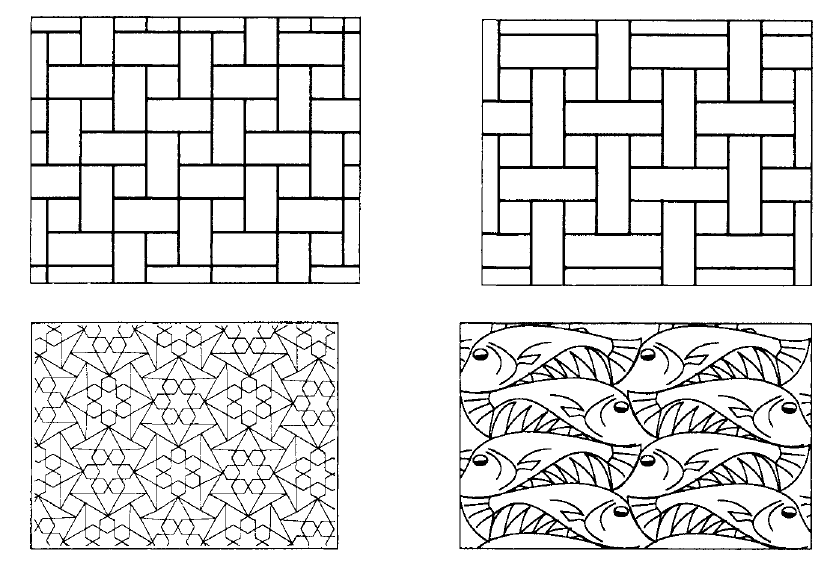
\includegraphics[width=0.45\textwidth]{artin-algebra-2e-ch06-ex-6.3-patterns.png}

{\scriptsize 图（Ex.~6.3）：左上 $p4$，右上 $p4g$，左下 $p6m$，右下 $pm$。}
\end{column}
\begin{column}{0.51\textwidth}
\key{详解（局部原则）}：设 $1\ne g\in G_x$。平面等距若保向且有不动点，必是绕 $x$ 的旋转；若反向且有不动点，必是反射；平移与滑移反射没有不动点。故 $x$ 只能是旋转中心或镜轴上的点。又 $G_x$ 是 $O(2)$ 的有限子群：若 $x$ 不在任何镜轴上，则 $G_x$ 只含旋转，$G_x\cong C_n$（$n$ 为该点的旋转阶）；一般镜轴点 $G_x\cong C_2$；若 $n$ 重旋转中心同时在两组镜轴的交点上，则 $G_x\cong D_n$。于是只需逐图找出旋转中心与镜轴。
\end{column}
\end{columns}
\end{frame}

\begin{frame}[t]{四、随机复习 4/15：G157 四个图案的稳定化子（下）}
\scriptsize
\textbf{左上 $p4$（点群 $C_4$，无镜轴）}：四重中心 $G_x=C_4=\langle r\rangle$，$r$ 为 $90^\circ$ 旋转；相邻四重中心连线的中点是二重中心，$G_x=C_2=\langle r^2\rangle$；其余点稳定化子平凡。

\textbf{右上 $p4g$（点群 $D_4$）}：四重中心不在镜轴上，$G_x=C_4$；二重中心恰为两组镜轴的交点，$G_x=D_2=\langle r^2,s_1,s_2\rangle$，其中 $s_1,s_2$ 为两条互相垂直的镜轴反射，且 $s_1s_2=r^2$（两个垂直反射之积是半转）；一般镜轴点 $G_x=C_2$；只在滑移轴上（不在镜轴上）的点稳定化子平凡。若四重中心恰在镜轴交点（即 $p4m$，本图不是），则 $G_x=D_4$。

\textbf{左下 $p6m$（点群 $D_6$）}：六重中心 $G_x=D_6$、三重中心 $G_x=D_3$、二重中心 $G_x=D_2$（旋转部分分别为 $C_6,C_3,C_2$，且均有镜轴通过；阶为 $12,6,4$）；一般镜轴点 $G_x=C_2$；其余点平凡。

\textbf{右下 $pm$（点群 $D_1$）}：无旋转中心；恰在水平镜轴上的点 $G_x=C_2=\langle s\rangle$；轴外点平凡（$pm$ 的保向部分只有平移）。

\starpt{}易错：滑移反射与平移没有不动点，不能算作“稳定子非平凡”；镜轴点要排除交点（交点稳定化子更大）；稳定化子只看该点附近被哪些群元固定，与整个图案的点群不同。
\end{frame}

% ---------------------------------------------------------- 5/15 G181
\begin{frame}[t]{四、随机复习 5/15：G181 对偶多面体的对称群同构}
\label{ex:G181}
\scriptsize
\begin{block}{\footnotesize 题面（\ex{G181}；Artin 2e, Ch.~6, §12, Ex.~12.1，印刷 p.~192 / PDF p.~204）}
解释为什么正十二面体与正二十面体的对称群同构。
\end{block}
\key{思路}：两者互为对偶：一者的面心是另一者的顶点。正交对称置换面，于是置换面心；两次对偶回到原多面体，故两个方向的映射互逆。

\key{详解}：把正十二面体 $D$ 同心放在原点，面为 $F_1,\dots,F_{12}$，面心为 $c_i$。$\{c_i\}$ 的凸包是正二十面体 $I$。设 $g\in\operatorname{Sym}(D)$。因 $D$ 有界，$g$ 固定其重心即原点，故 $g$ 是绕原点的正交变换；它置换面，$g(F_i)=F_{\sigma(i)}$，故
\[ g(c_i)=c_{\sigma(i)}\quad\Longrightarrow\quad g\bigl(\operatorname{conv}\{c_i\}\bigr)=\operatorname{conv}\{g c_i\}=\operatorname{conv}\{c_i\}, \]
即 $g$ 把 $I$ 送到自身：$g\in\operatorname{Sym}(I)$。于是有映射 $\varphi:\operatorname{Sym}(D)\to\operatorname{Sym}(I)$，$\varphi(g)=g$（同一个正交变换）；$\varphi(gh)$ 与 $\varphi(g)\varphi(h)$ 是同一个复合变换，故 $\varphi$ 是同态。

\key{互逆}：对 $I$ 作同样构造，其对偶的顶点是 $I$ 的 $20$ 个面心，恰为 $D$ 的 $20$ 个顶点，凸包回到 $D$。故任何 $h\in\operatorname{Sym}(I)$ 置换 $I$ 的面、从而置换 $D$ 的顶点，于是 $h\in\operatorname{Sym}(D)$。两个方向的映射都是恒等对应，故 $\operatorname{Sym}(D)=\operatorname{Sym}(I)$（作为 $O(3)$ 的同一子群），特别地同构。

\key{验算}：$|\operatorname{Sym}(D)|=12\cdot10=120$（$12$ 个面，每面稳定化子 $D_5$ 阶 $10$）；$|\operatorname{Sym}(I)|=20\cdot6=120$（$20$ 个面，每面稳定化子 $D_3$ 阶 $6$），也等于 $12\cdot10$（$12$ 个顶点，每顶点稳定化子 $D_5$）。旋转子群也同构，阶 $60=12\cdot5=20\cdot3$；两者轴的重数相同：$6$ 条五重轴、$10$ 条三重轴、$15$ 条二重轴。
\end{frame}

% ---------------------------------------------------------- 6/15 G173
\begin{frame}[t]{四、随机复习 6/15：G173 $S_3$ 在四点上的作用（上）}
\label{ex:G173}
\scriptsize
\begin{block}{\footnotesize 题面（\ex{G173}；Artin 2e, Ch.~6, §11, Ex.~11.1，印刷 p.~192 / PDF p.~204）}
描述 $S_3$ 作用在一个四元集上的所有方式。
\end{block}
\key{思路}：按轨道分拆四点集。传递作用同构于在子群陪集上的作用，轨道大小即子群指数，必整除 $6$；不超过 $4$ 的可用轨道大小只有 $1,2,3$（不存在指数 $4$ 的子群），再把 $4$ 分拆。

\key{详解}：$S_3$ 的子群阶为 $1,2,3,6$，对应指数（即传递轨道大小）为 $6,3,2,1$：
\begin{center}
{\scriptsize
\begin{tabular}{@{}llll@{}}
\toprule
子群 & 指数 $=$ 轨道大小 & 共轭类 & 传递 $S_3$-集\\ \midrule
$S_3$ & $1$ & $1$ & 平凡作用\\
$A_3$ & $2$ & $1$ & 符号作用\\
三个二阶子群 $\langle(12)\rangle$ 等 & $3$ & $1$ & 自然作用（三点）\\
$\{1\}$ & $6$ & $1$ & 正则作用（六点，超界）\\ \bottomrule
\end{tabular}}
\end{center}
把 $4$ 写成取自 $\{1,2,3\}$ 的部分之和，只有 $1+1+1+1$、$2+1+1$、$2+2$、$3+1$ 四种。若存在大小为 $4$ 的轨道 $S_3/H$，则 $|H|=6/4\notin\mathbb Z$，矛盾，故不会出现单轨道四点作用。
\end{frame}

\begin{frame}[t]{四、随机复习 6/15：G173 $S_3$ 在四点上的作用（下）}
\scriptsize
\key{四个作用的具体表示}（记 $a=(123)$，$b=(12)$，四点为 $1,2,3,4$）：
\begin{center}
{\scriptsize
\begin{tabular}{@{}lcccc@{}}
\toprule
作用 & $\rho(a)$ & $\rho(b)$ & $\ker\rho$ & 轨道分拆\\ \midrule
$1+1+1+1$ & $\mathrm{id}$ & $\mathrm{id}$ & $S_3$ & $1|1|1|1$\\
$2+1+1$ & $\mathrm{id}$ & $(12)$ & $A_3$ & $2|1|1$\\
$2+2$ & $\mathrm{id}$ & $(12)(34)$ & $A_3$ & $2|2$\\
$3+1$ & $(123)$ & $(12)$ & $\{1\}$ & $3|1$\\ \bottomrule
\end{tabular}}
\end{center}
\key{核对}：$2+1+1$ 中 $\{1,2\}$ 的轨道大小 $=|S_3|/|A_3|=6/2=2$；$3+1$ 中点 $1$ 的稳定化子是 $\langle(23)\rangle$，指数 $6/2=3$，且 $4$ 被固定；$2+2$ 是符号作用的两份不交并。四个核分别为 $S_3,A_3,A_3,\{1\}$，互不相同，故四个作用互不等价。

\key{唯一性}：传递作用满足 $S_3/H\cong S_3/H'$ 当且仅当 $H,H'$ 共轭。上述四类子群各自恰为一个共轭类（$S_3,A_3,\{1\}$ 正规，三个二阶子群相互共轭），所以每个可用传递型唯一；非传递型由这些传递型作不交并唯一确定。因此四种分拆给出且仅给出四种作用。$\square$
\end{frame}

% ---------------------------------------------------------- 7/15 G153
\begin{frame}[t]{四、随机复习 7/15：G153 十七个平面晶体群（上）}
\label{ex:G153}
\scriptsize
\begin{block}{\footnotesize 题面（\ex{G153}；Artin 2e, Ch.~6, §6, Ex.~6.6，印刷 p.~190 / PDF p.~202；Fig.~6.6.2，印刷 p.~174 / PDF p.~186）}
证明 Figure 6.6.2 中各图形的对称群穷尽了所有可能。
\end{block}
\key{思路}：设 $L$ 为平移格、$\overline G$ 为点群，得到正合列；晶体限制把 $\overline G$ 压到 $C_n$ 或 $D_n$（$n\in\{1,2,3,4,6\}$）；再按每种不变格分类点群生成元的提升，模平移与原点平移即得有限多种。

\key{详解（正合列）}：$\overline G$ 是 $G$ 的正交部分像，$L$ 是平移子群（平移 $t_v\in G$ 当且仅当 $L+v=L$，即 $v\in L$）：
\[ 1\longrightarrow L\longrightarrow G\longrightarrow\overline G\longrightarrow 1. \]
\key{晶体限制}：设点群中出现旋转角 $\theta$ 的正交部分 $Q$。因 $L=\ker(G\to O(2))$ 正规，$Q(L)=L$；在 $L$ 的整基下 $Q$ 的矩阵 $A\in GL_2(\mathbb Z)$，故迹 $\operatorname{tr}A=2\cos\theta\in\mathbb Z$；又 $|2\cos\theta|\le2$，于是
\[ 2\cos\theta\in\{-2,-1,0,1,2\}\ \Longrightarrow\ \theta\in\{180^\circ,120^\circ,90^\circ,60^\circ,0^\circ\}, \]
即旋转阶 $n\in\{1,2,3,4,6\}$。反向部分至多再乘一个镜射，故 $\overline G=C_n$ 或 $D_n$，$n\in\{1,2,3,4,6\}$。

\key{适配格}：$C_1,C_2$ 用斜格；$D_1,D_2$ 用矩形或中心矩形格；$4$ 阶用正方格；$3,6$ 阶用三角格。
\end{frame}

\begin{frame}[t]{四、随机复习 7/15：G153 十七个平面晶体群（下）}
\scriptsize
\begin{columns}[T]
\begin{column}{0.29\textwidth}
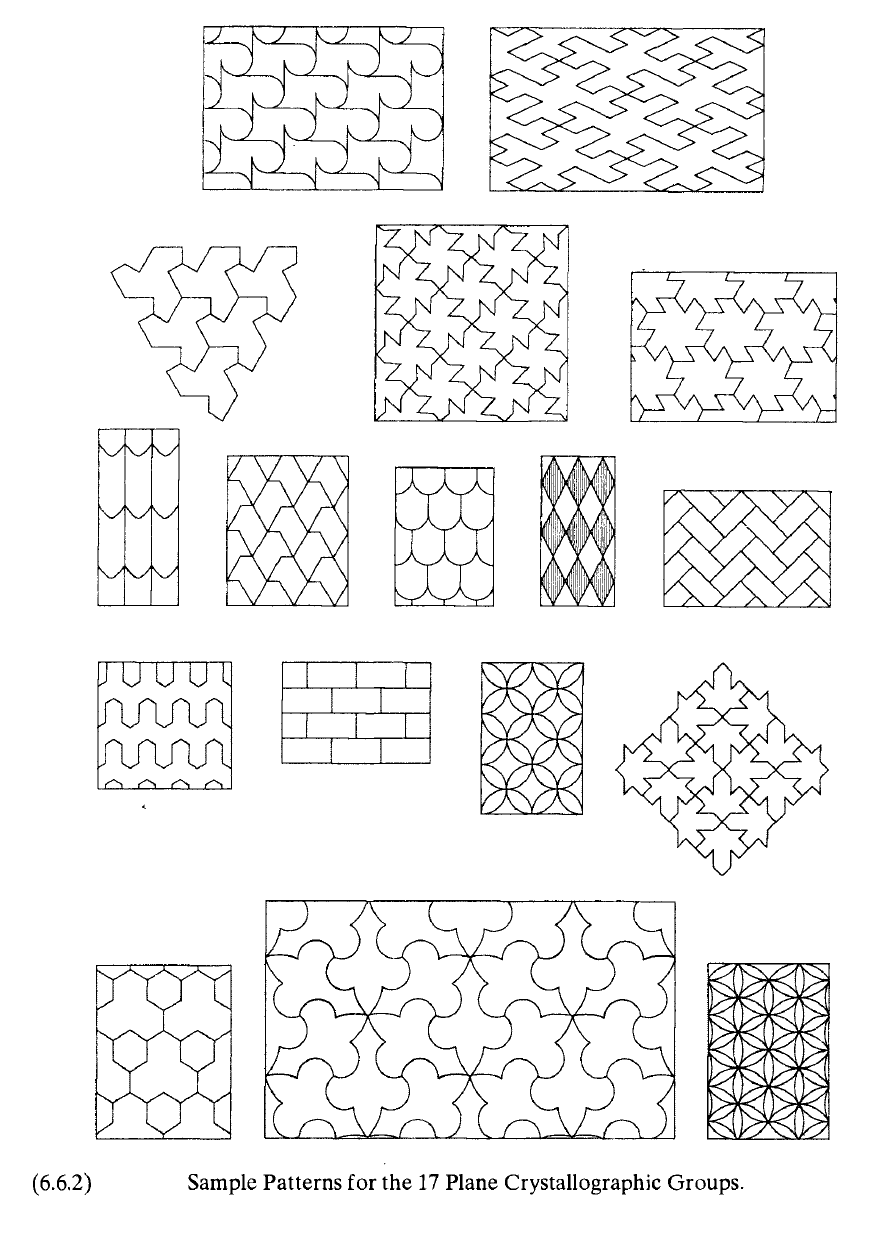
\includegraphics[width=0.99\textwidth]{artin-algebra-2e-ch06-fig-6.6.2.png}

{\scriptsize 图 6.6.2：$17$ 个平面晶体群的样本图案（逐行见右栏）。}
\end{column}
\begin{column}{0.68\textwidth}
\key{提升计算}：设点群元 $q\in O(2)$ 的提升为 $g=t_uq$。换提升 $t_vg$（$v\in L$）只改 $u$ 模 $L$；换原点 $c$ 时 $t_cgt_c^{-1}=t_{u+(I-q)c}\,q$。故 $u$ 可在模 $L$ 的有限个类中调整，只需在 $L/2L$ 一类上解 $C_n$ 或 $D_n$ 的生成关系。
\begin{center}
{\scriptsize
\begin{tabular}{@{}llr@{}}
\toprule
点群 & 仿射类型 & 个数\\ \midrule
$C_n$（$n=1,2,3,4,6$） & $p1,p2,p3,p4,p6$ & $5\cdot1$\\
$D_1$ & $pm,pg,cm$ & $3$\\
$D_2$ & $pmm,pmg,pgg,cmm$ & $4$\\
$D_3$ & $p3m1,p31m$ & $2$\\
$D_4$ & $p4m,p4g$ & $2$\\
$D_6$ & $p6m$ & $1$\\ \bottomrule
\end{tabular}}
\end{center}
循环情形：旋转提升有不动点，把原点移到该点后 $u=0$，每种 $n$ 只剩 $1$ 型。二面体情形：各镜射方向的提升可为真镜射或“强制半滑移”，按 $u$ 的 $L/2L$ 类分类：$D_1$ 得 $3$ 型；$D_2$ 的两族镜射各有镜/滑选择且乘积须为半转，得 $4$ 型；三角格上 $D_3$ 有两种镜轴安放（$p3m1,p31m$）；正方格上 $D_4$ 有“镜轴过四重中心”与“错位镜/滑”两种（$p4m,p4g$）；$D_6$ 只有 $p6m$。

\key{计数}：$1+1+1+1+1+3+4+2+2+1=17$。图 6.6.2 的 $17$ 个图案按行实现各行类型：$p1,p2$／$p3,p4,p6$／$pm,pg,cm,pmm,pmg$／$pgg,cmm,p4m,p4g$／$p3m1,p31m,p6m$，故这些对称群穷尽全部平面晶体群。
\end{column}
\end{columns}
\end{frame}

% ---------------------------------------------------------- 8/15 G175
\begin{frame}[t]{四、随机复习 8/15：G175 作用核是正规子群}
\label{ex:G175}
\scriptsize
\begin{block}{\footnotesize 题面（\ex{G175}；Artin 2e, Ch.~6, §11, Ex.~11.3，印刷 p.~192 / PDF p.~204）}
设群 $G$ 作用在集合 $S$ 上，$H=\{g\in G:gs=s\ \text{对一切}\ s\in S\}$。证明 $H$ 是 $G$ 的正规子群。
\end{block}
\key{思路}：作用给出同态 $\rho:G\to\operatorname{Sym}(S)$，$H=\ker\rho$；核必正规。再用作用律直接验证共轭不变。

\key{详解}：定义 $\rho(g)(s)=gs$。由作用律 $(gh)s=g(hs)$ 得
\[ \rho(gh)(s)=(gh)s=g(hs)=\rho(g)\bigl(\rho(h)(s)\bigr)=(\rho(g)\circ\rho(h))(s), \]
故 $\rho$ 是同态，且 $\rho(1)=\mathrm{id}_S$、$\rho(g^{-1})=\rho(g)^{-1}$。其次
\[ g\in\ker\rho\iff\rho(g)=\mathrm{id}_S\iff gs=s\ \text{对一切}\ s\in S\iff g\in H, \]
所以 $H=\ker\rho$。

\key{核正规}：对 $g\in G$、$h\in H$，$\rho(ghg^{-1})=\rho(g)\rho(h)\rho(g)^{-1}=\rho(g)\mathrm{id}\rho(g)^{-1}=\mathrm{id}$，故 $ghg^{-1}\in H$。

\key{不用同态的直接验证}：$h\in H$、$g\in G$、$s\in S$ 时
\[ (ghg^{-1})s=g\bigl(h(g^{-1}s)\bigr)=g(g^{-1}s)=s, \]
最后一步用了 $h$ 固定一切点（包括 $g^{-1}s$），故 $ghg^{-1}\in H$。又 $1\in H$；$h_1,h_2\in H$ 时 $(h_1h_2)s=h_1(h_2s)=h_1s=s$；由 $hs=s$ 作用 $h^{-1}$ 得 $s=h^{-1}s$，故 $H\le G$。

\key{具体例子}：$S_3$ 在两点上由符号作用时 $H=A_3\triangleleft S_3$，指数 $2$；$S_3$ 在三点上自然作用时 $H=\{1\}$。一般地，作用忠实当且仅当 $H=\{1\}$。
\end{frame}


\begin{frame}[t]{四、随机复习 9/15：G170 $D_3$ 在三元子集上的轨道（上）}
\label{ex:G170}
\scriptsize
\begin{block}{\footnotesize 题面 \ex{G170}（Artin 2e, Ch.~6, \S\,10, Ex.~10.1；印刷 p.~192 / PDF p.~204）}
Determine the orders of the orbits for left multiplication on the set of subsets of order $3$ of $D_3$.\\
求左乘作用在 $D_3$ 的三元子集集合上的各轨道阶数。
\end{block}
\key{思路}：左乘是自由作用，故三元子集 $X$ 的轨道大小 $=6/|\mathrm{Stab}(X)|$；只需把 $|\mathrm{Stab}(X)|\in\{1,2,3,6\}$ 逐个判定。
\key{详解}（一）稳定化子的可能阶数。
\begin{itemize}\setlength{\itemsep}{1pt}\setlength{\parsep}{0pt}
\item 记 $R=\langle r\rangle=\{1,r,r^2\}\le D_3$ 为 $3$ 阶旋转子群，则 $D_3=R\cup sR$，$|D_3|=6$。
\item 左乘无不动点：$gx=x\Rightarrow g=1$。故 $D_3$ 在自身上的左乘作用既自由又传递。
\item 对三元子集 $X$，轨道—稳定化子定理给出 $|D_3\cdot X|=6/|\mathrm{Stab}(X)|$；又 $|\mathrm{Stab}(X)|\mid 6$，故 $|\mathrm{Stab}(X)|\in\{1,2,3,6\}$。
\item $|\mathrm{Stab}(X)|=6$ 不可能：则 $X$ 为 $D_3$-不变集，而 $D_3$ 在自身上传递，不变子集只能是 $\varnothing$ 或整个 $D_3$（$6$ 元），与 $|X|=3$ 矛盾。
\item $|\mathrm{Stab}(X)|=2$ 不可能：设对合 $s'\in\mathrm{Stab}(X)$。由 $s'x\ne x$，$\langle s'\rangle$ 的轨道都是二元对 $\{x,s'x\}$；$s'$-不变集必为这些对的并，大小是偶数，与 $|X|=3$ 矛盾。
\item 具体写出：以 $s$ 为例，左乘 $s$ 的三条轨道为 $\{1,s\}$、$\{r,sr\}$、$\{r^2,sr^2\}$（因 $s\cdot r=sr,\ s\cdot sr=s^2r=r$）。故任何 $s$-不变集的大小只能是 $0,2,4,6$，绝不是 $3$。
\item \starpt 结论：没有三元子集被对合固定（对合只固定二元子集，如 $X=\{1,s\}$）；于是只剩 $|\mathrm{Stab}(X)|\in\{1,3\}$。
\end{itemize}
\end{frame}

\begin{frame}[t]{四、随机复习 9/15：G170 $D_3$ 在三元子集上的轨道（下）}
\scriptsize
\key{详解}（二）阶 $3$ 的情形与轨道计数。
\begin{itemize}\setlength{\itemsep}{1pt}\setlength{\parsep}{0pt}
\item $D_3$ 的 $3$ 阶子群只有 $R$；$X$ 被 $R$ 稳定 $\iff X$ 是 $R$ 左乘轨道的并。
\item $R$ 在 $D_3$ 上左乘的轨道恰是 $R$ 与 $sR$（各 $3$ 元）。故只有 $X=R$、$X=sR$ 两个三元子集被 $R$ 稳定，且 $\mathrm{Stab}(R)=R$（$gR=R\iff g\in R$）。
\item $D_3\cdot R=\{gR:g\in D_3\}=\{R,sR\}$，于是
\[ |D_3\cdot R|=\frac{|D_3|}{|\mathrm{Stab}(R)|}=\frac63=2 .\]
\item 其余 $\binom63-2=18$ 个子集稳定化子平凡，轨道大小 $6/1=6$，故有 $18/6=3$ 个轨道。
\item 四个轨道的大小为 $2,6,6,6$；校验 $2+6+6+6=20=\binom63$。
\end{itemize}
\key{验算}（穷举核对）：取 $D_3=\{1,r,r^2,s,sr,sr^2\}$，对全部 $20$ 个三元子集按左乘闭包逐个求轨道，得 $4$ 个轨道、大小为 $[2,6,6,6]$；稳定化子阶的直方图为 $\{1{:}18,\;3{:}2\}$，两个阶 $3$ 稳定化子的子集正是 $R$ 与 $sR$。
\starpt 易错点：(i) 漏掉 $|\mathrm{Stab}|=6$ 的排除，会误以为存在 $1$ 元轨道；(ii) 把 $R$ 与 $sR$ 当成两个不同的轨道——它们同属一个 $2$ 元轨道；(iii) 把“对合没有不动点”误记为“对合固定不了任何子集”：它固定二元子集，只是固定不了三元子集。
\end{frame}

\begin{frame}[t]{四、随机复习 10/15：G109 三角形花边的对称群（上）}
\label{ex:G109}
\scriptsize
\begin{block}{\footnotesize 题面 \ex{G109}（Artin 2e, Ch.~6, \S\,5, Ex.~5.5；印刷 p.~188 / PDF p.~200；图案即印在题内）}
Prove that the group of symmetries of the following frieze pattern is isomorphic to the direct product $C_2\times C_\infty$ of a cyclic group of order $2$ and an infinite cyclic group.
\end{block}
\key{思路}：取最小水平平移 $t$ 与水平轴反射 $r$，验证 $r^2=1$、$rt=tr$；再证明造不出别的对称（水平轴唯一，顶点集周期为 $a$）。
\begin{columns}[T]
\begin{column}{0.55\textwidth}
\key{详解}（一）两条基本对称。取花边的水平轴为 $x$ 轴、相邻三角形间距 $a>0$，则
\[ t(x,y)=(x+a,y),\qquad r(x,y)=(x,-y). \]
具体地，第 $k$ 个三角形的顶点为 $\big((k+\tfrac12)a,\,0\big)$、底边端点为 $\big((k+1)a,\,\pm h\big)$；于是 $t$ 把第 $k$ 个送到第 $k+1$ 个，$r$ 固定顶点而互换两个底边端点（故把每个三角形映到自身）。
图案是这些三角形的并，故任一对称必把三角形集合映到自身；又 $t^k=\mathrm{id}\iff k=0$（$t^k$ 把顶点 $\big(\tfrac12a,0\big)$ 移到 $\big((k+\tfrac12)a,0\big)$），故 $\langle t\rangle\cong C_\infty$。
\end{column}
\begin{column}{0.43\textwidth}
\centering

\includegraphics[width=0.42\textwidth]{artin-algebra-2e-ch06-ex-5.5-frieze.png}\\
{\tiny 图案：$7$ 个全等三角形排成一列，顶点朝左、竖直底边在右；顶点与底边中点都落在同一水平轴 $\ell$ 上。}
\end{column}
\end{columns}
\key{详解}（二）关系与生成。
\[ r^2=1,\qquad rt(x,y)=r(x+a,y)=(x+a,-y)=tr(x,y). \]
即 $rt=tr$（关于水平轴的反射保持水平平移方向，不求逆）。于是 $t^kr=rt^k$，所有 $t^k$、$rt^k$（$k\in\mathbb Z$）都是对称。
\end{frame}

\begin{frame}[t]{四、随机复习 10/15：G109 三角形花边的对称群（下）}
\scriptsize
\key{详解}（三）穷尽性。任一对称 $\sigma$ 把图案映到自身，故把 $\ell$ 映到自身（图案的最小凸包是 $\ell$ 两侧的窄带，$\ell$ 是其中轴），从而把水平方向映到水平方向，线性部分只能是 $\mathrm{diag}(\pm1,\pm1)$ 四种：
\begin{itemize}\setlength{\itemsep}{1pt}\setlength{\parsep}{0pt}
\item $I$：$\sigma(x,y)=(x+c,y)$ 是平移。顶点集 $\{((k+\frac12)a,\,0)\}$ 的周期为 $a$，故 $c=ka$，$\sigma=t^k$。
\item $\mathrm{diag}(1,-1)$：$\sigma(x,y)=(x+c,-y)=rt^{c/a}$，同样 $c=ka$，即 $\sigma=rt^k$——轴为 $\ell$ 的滑移反射，$k=0$ 时退化为纯反射 $r$。
\item $\mathrm{diag}(-1,1)$：竖直轴上的反射或滑移 $(-x+c,\,y+e)$，会把“顶点朝左”变成“顶点朝右”，而图中三角形全朝左；且图案无竖直周期，故 $e=0$。
\item $-I$：半转 $(c-x,-y+e)$，同样把“顶点朝左”转成“顶点朝右”。后两种都不可能。
\end{itemize}
于是对称群恰为 $G=\{t^k\}\cup\{rt^k\}$：$t^k$ 是平移（保向），$rt^k$ 是反定向元（$k=0$ 为纯反射，$k\ne0$ 为滑移反射）。特别地
\[ rt^k(x,y)=(x+ka,-y)=t^kr(x,y),\qquad k\in\mathbb Z, \]
与 $rt=tr$ 一致，故 $G$ 交换。
\key{详解}（四）识别为直积。令 $\langle t\rangle$ 与 $\langle r\rangle$ 为两个子群：
\begin{itemize}\setlength{\itemsep}{1pt}\setlength{\parsep}{0pt}
\item $\langle t\rangle\cong C_\infty$（$t^k=1\iff k=0$），$\langle r\rangle\cong C_2$；
\item $rt=tr$，$\langle t\rangle\cap\langle r\rangle=\{1\}$（$r$ 反定向，$t^k$ 保定向），二者生成 $G$；
\item 每个元素唯一写成 $t^kr^\varepsilon$（$\varepsilon\in\{0,1\}$），且乘法逐分量：
\[ t^kr^\varepsilon\cdot t^{k'}r^{\varepsilon'}=t^{k+k'}r^{\varepsilon+\varepsilon'}, \]
与 $C_2\times C_\infty$ 中 $(\varepsilon,k)\cdot(\varepsilon',k')=(\varepsilon+\varepsilon',k+k')$ 完全一致。故 $G\cong C_2\times C_\infty$；特别地 $G$ 交换，$rtr=t$。
\end{itemize}
\starpt 易错点：勿把本题的 $r$（水平轴反射）与 G16 图 6.1.7 的 $v$（竖直轴反射）混淆——竖直反射才对水平平移取逆（$vtv=t^{-1}$），那给出半直积而非直积。这正是本题 $C_2\times C_\infty$ 与 6.1.7 的 $D_\infty$ 的差别。
\end{frame}

\begin{frame}[t]{四、随机复习 11/15：LA298 双侧矩阵等价的轨道（上）}
\label{ex:LA298}
\scriptsize
\begin{block}{\footnotesize 题面 \ex{LA298}（Artin 2e, Ch.~6, \S\,7, Ex.~7.9；印刷 p.~191 / PDF p.~203）}
(a) 设 $S=\mathbb R^{m\times n}$、$G=GL_m(\mathbb R)\times GL_n(\mathbb R)$，证明 $(P,Q)*A=PAQ^{-1}$ 定义了 $G$ 在 $S$ 上的一个作用。\quad
(b) 描述 $S$ 的 $G$-轨道分解。\quad
(c) 设 $m\le n$，求矩阵 $[I_m\mid 0]$ 的稳定化子。
\end{block}
\key{思路}：逐条验作用公理（要点是 $Q^{-1}$ 的顺序）；用可逆行、列变换化标准形；对 (c) 按 $m$ 与 $n-m$ 分块解 $PA_0=A_0Q$。
\key{详解}(a)：单位元作用平凡：$(I_m,I_n)*A=I_mAI_n^{-1}=A$。再看乘法（$G$ 中按分量相乘）：
\[
(P_1,Q_1)*\big((P_2,Q_2)*A\big)=P_1\big(P_2AQ_2^{-1}\big)Q_1^{-1}
=P_1P_2\,A\,Q_2^{-1}Q_1^{-1}=(P_1P_2,\,Q_1Q_2)*A,
\]
最后一步用了 $(Q_1Q_2)^{-1}=Q_2^{-1}Q_1^{-1}$——逆把顺序倒回来，恰好抵消左边新添的 $Q_1^{-1}$。故这是左作用。
\key{详解}(b)：$P$ 左乘、$Q^{-1}$ 右乘都是可逆的行、列变换，秩不变，故每条轨道落在某个秩层内。反之，秩为 $r$ 的 $A$ 经行、列变换可化为标准形
\[ A_r=\begin{pmatrix}I_r&0\\0&0\end{pmatrix}_{m\times n}, \]
即存在可逆 $P,Q$ 使 $PAQ=A_r$。故轨道恰是各秩层 $\{A:\operatorname{rank}A=r\}$，$r=0,1,\dots,\min(m,n)$，共 $\min(m,n)+1$ 个。例如 $m=2,n=3$ 时有 $r=0,1,2$ 三个轨道。
\key{验算}（$m=2,n=3$ 的具体化）：取 $\operatorname{rank}A=2$ 的
\[
A=\begin{pmatrix}1&2&3\\2&4&7\end{pmatrix}
\xrightarrow{R_2-2R_1}\begin{pmatrix}1&2&3\\0&0&1\end{pmatrix}
\xrightarrow[\ C_3-3C_1]{\ C_2-2C_1}\begin{pmatrix}1&0&0\\0&0&1\end{pmatrix}
\xrightarrow{C_2\leftrightarrow C_3}\begin{pmatrix}1&0&0\\0&1&0\end{pmatrix}=A_2,
\]
其中行变换由 $P=\begin{pmatrix}1&0\\-2&1\end{pmatrix}$ 给出，列变换即右乘某个可逆阵 $C$；取 $Q=C^{-1}$ 便得 $(P,Q)*A=PAQ^{-1}=A_2$。
\end{frame}

\begin{frame}[t]{四、随机复习 11/15：LA298 双侧矩阵等价的轨道（下）}
\scriptsize
\key{详解}(c)：设 $A_0=[I_m\mid 0]$，把 $Q$ 按 $m$、$n-m$ 分块：$Q=\begin{pmatrix}Q_{11}&Q_{12}\\ Q_{21}&Q_{22}\end{pmatrix}$，其中 $Q_{11}$ 为 $m\times m$、$Q_{22}$ 为 $(n-m)\times(n-m)$。稳定化子方程与等价变形：
\[
PA_0Q^{-1}=A_0\iff PA_0=A_0Q\iff [\,P\mid 0\,]=[\,Q_{11}\mid Q_{12}\,].
\]
（$A_0Q$ 就是 $Q$ 的前 $m$ 行。）逐块比较：$Q_{11}=P$，$Q_{12}=0$。于是
\[
Q=\begin{pmatrix}P&0\\ C&D\end{pmatrix},\qquad \det Q=\det P\cdot\det D,
\]
故 $Q$ 可逆 $\iff P\in GL_m(\mathbb R)$、$D\in GL_{n-m}(\mathbb R)$，而 $C=Q_{21}\in\mathbb R^{(n-m)\times m}$ 任意。因此
\[
\mathrm{Stab}(A_0)=\Big\{\Big(P,\begin{pmatrix}P&0\\ C&D\end{pmatrix}\Big):P\in GL_m(\mathbb R),\;D\in GL_{n-m}(\mathbb R),\;C\in\mathbb R^{(n-m)\times m}\Big\}.
\]
\key{验算}：取 $m=1,n=2$，$P=(p)$，$Q=\begin{pmatrix}p&0\\ c&d\end{pmatrix}$，$p,d\ne0$。则 $Q^{-1}=\begin{pmatrix}1/p&0\\ -c/(pd)&1/d\end{pmatrix}$，$[1\ 0]Q^{-1}=[1/p\ 0]$，乘以 $p$ 得 $[1\ 0]=A_0$。\\[1pt]
\key{验算}（维数）：$\dim G-\dim\mathrm{Stab}=m^2+n^2-\big[m^2+m(n-m)+(n-m)^2\big]=mn$，恰等于秩 $m$ 轨道的维数 $m(m+n-m)=mn$。
\starpt 易错点：$(Q_1Q_2)^{-1}=Q_2^{-1}Q_1^{-1}$ 的顺序若写反，(a) 不成立；$(P,Q)*A=PAQ$ 或 $PAQ^{\mathsf T}$ 都不是作用（见 LA300）。
\end{frame}

\begin{frame}[t]{四、随机复习 12/15：G16 三类平面图案的对称群（上）}
\label{ex:G16}
\scriptsize
\begin{block}{\footnotesize 题面 \ex{G16}（Artin 2e, Ch.~6, \S\,1, Ex.~1.1；印刷 p.~188 / PDF p.~200；图 6.1.4--6.1.7 在印刷 p.~155 / PDF p.~167）}
Determine all symmetries of Figures 6.1.4, 6.1.6 and 6.1.7.（三幅图案都向左右无限延伸。）
\end{block}
\key{思路}：先找最小步长的生成元，再说明“一个基本图形的像与朝向”唯一决定整条对称，从而列表穷尽。
约定：$a>0$ 为相邻基本位置的水平间距；$t_c$ 为水平平移 $c$；$r$ 为关于水平基线 $\ell$ 的反射。先看 6.1.4（滑移对称）。
\begin{columns}[T]
\begin{column}{0.55\textwidth}
取 $g=rt_a$（$r,t_a$ 可交换，见下）：先关于 $\ell$ 反射、再平移 $a$。上叶附着点在 $2ka$、朝右上；下叶在 $(2k+1)a$、朝右下，故 $g$ 把每片上叶送下一片下叶。又
\[ rt_ar(x,y)=r(x+a,-y)=(x+a,y)=t_a(x,y), \]
即 $rt_ar=t_a$，于是
\[ g^2=rt_art_a=t_at_a=t_{2a}. \]
故 $g^{2k}=t_{2ka}$ 是平移，$g^{2k+1}$ 是滑移反射。
\end{column}
\begin{column}{0.43\textwidth}
\centering
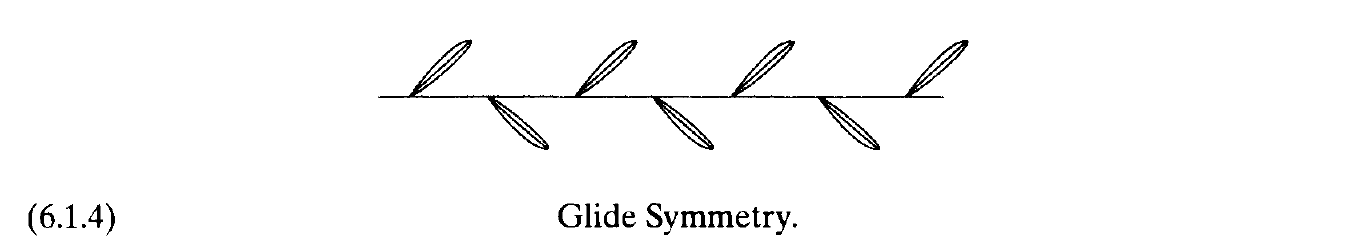
\includegraphics[width=0.30\textwidth]{artin-algebra-2e-ch06-fig-6.1.4.png}\\
{\tiny 图 6.1.4：叶片在水平基线两侧交错，上叶朝右上、下叶朝右下，附着点相隔 $a$。}
\end{column}
\end{columns}
\key{穷尽}(6.1.4)：纯平移必须保住上、下排，故周期是 $2a$，只有 $t_{2ka}=g^{2k}$；关于 $\ell$ 的反射必须配 $a$ 的奇数倍平移才落到真实叶片上，得 $g^{2k+1}$；竖直反射会把“朝右上”变成“朝左上”，半转把它变成“朝左下”，图中都没有。故 $\mathrm{Sym}(6.1.4)=\langle g\rangle\cong\mathbb Z$。
\key{接着} 6.1.6（平移加半转）。
\begin{columns}[T]
\begin{column}{0.55\textwidth}
$t$：平移一个“happy”（周期 $a$）；$s$：关于相邻两词交接处的半转（$y$ 的下降部与下一个 $h$ 的上升部互换），中心每隔 $a$ 出现一个。取 $t(x,y)=(x+a,y)$、$s(x,y)=(-x,-y)$，则
\[ s^2=1,\qquad sts=t^{-1}, \]
且所有 $t^n$、$t^ns$ 都是对称（后者是各旋转中心处的半转）。
\end{column}
\begin{column}{0.43\textwidth}
\centering
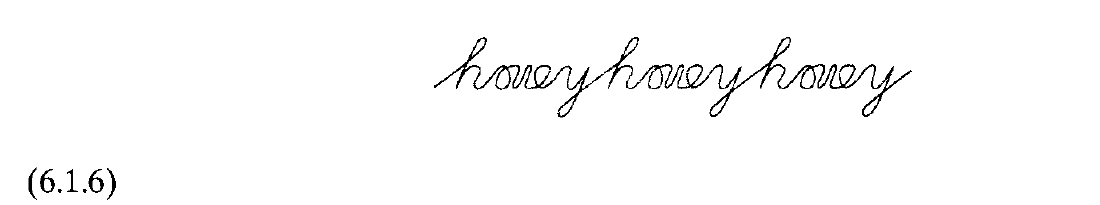
\includegraphics[width=0.30\textwidth]{artin-algebra-2e-ch06-fig-6.1.6.png}\\
{\tiny 图 6.1.6：“happy”连写重复；词与词的交接处是 $180^\circ$ 旋转中心。}
\end{column}
\end{columns}
\end{frame}

\begin{frame}[t]{四、随机复习 12/15：G16 三类平面图案的对称群（下）}
\scriptsize
\key{穷尽}(6.1.6)：任一对称把图案所在水平带的中线（水平方向）映到自身，故其线性部分只能是 $\mathrm{diag}(\pm1,\pm1)$ 四种，逐种排除：
(i) $I$：$(x,y)\mapsto(x+c,y)$ 是平移，词界须映到词界，故 $c\in a\mathbb Z$，得 $t^n$；
(ii) $-I$：半转，中心在词界处，得 $t^ns$；
(iii) $\mathrm{diag}(-1,1)$：竖直反射 $(x,y)\mapsto(c-x,y)$，会把“happy”反写成“yppah”；
(iv) $\mathrm{diag}(1,-1)$：水平反射或滑移 $(x,y)\mapsto(x+c,-y)$，会把字上下颠倒（$h$ 的上升部落到基线下方）。后两种图中都没有。故
$\mathrm{Sym}(6.1.6)=\langle t,s\mid s^2=1,\ sts=t^{-1}\rangle\cong D_\infty$。
\key{详解} 6.1.7（竖直反射加入）。记 $g$ 为关于水平轴的滑移反射（把正立小人送到相邻的倒立小人），$v$ 为关于某个小人竖直中线的反射。取坐标使
\[ g(x,y)=(x+a,-y),\qquad v(x,y)=(-x,y), \]
则 $v^2=1$，$g^2=t_{2a}$，且用 $vrv=r$、$vt_av=t_{-a}$ 得
\[ vgv=(vrv)(vt_av)=rt_{-a}=g^{-1}. \]
\begin{columns}[T]
\begin{column}{0.56\textwidth}
四类元素（$k\in\mathbb Z$）：
\begin{itemize}\setlength{\itemsep}{0pt}\setlength{\parsep}{0pt}
\item $g^{2k}=t_{2ka}$：平移；
\item $g^{2k+1}$：水平滑移反射；
\item $g^{2k}v$：竖直线 $x=ka$ 上的反射（过小人）；
\item $g^{2k+1}v$：中心在 $\big((2k+\tfrac12)a,\,0\big)$ 的半转（相邻两图形正中）。
\end{itemize}
穷尽：按线性部分分类——$I$ 给平移 $t_c$，须保图形朝向，故 $c\in2a\mathbb Z$，即 $g^{2k}$；$\mathrm{diag}(1,-1)$ 给水平轴上的反射或滑移，但同一点上下不同时出现图形，故只能是滑移 $g^{2k+1}$；$\mathrm{diag}(-1,1)$ 给竖直反射 $g^{2k}v$；$-I$ 给半转 $g^{2k+1}v$。故 $\mathrm{Sym}(6.1.7)=\langle g,v\mid v^2=1,\ vgv=g^{-1}\rangle\cong D_\infty$。
\end{column}
\begin{column}{0.42\textwidth}
\centering
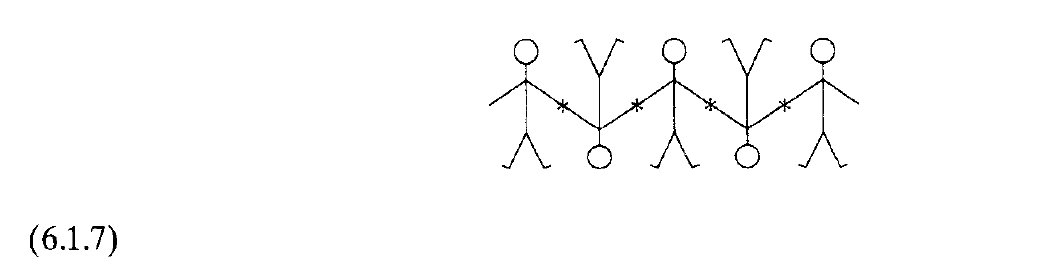
\includegraphics[width=0.30\textwidth]{artin-algebra-2e-ch06-fig-6.1.7.png}\\
{\tiny 图 6.1.7：正立、倒立小人交替（纯平移周期 $2a$），斜线带 $\ast$ 标出相邻连接；竖直镜线过小人，半转中心在相邻两图形正中。}
\end{column}
\end{columns}
\key{对照}：6.1.4 得 $\mathbb Z$（只有平移与滑移）；6.1.6 与 6.1.7 都同构于 $D_\infty$，但几何实现不同——6.1.6 的二阶元全是半转（点群 $\{1,-1\}$），6.1.7 的二阶元兼有竖直反射与半转（点群为 Klein 四元群）。\starpt 抽象同构不代表图案等价。
\end{frame}

\begin{frame}[t]{四、随机复习 13/15：G151 点群 $D_1$ 的平面晶体群（上）}
\label{ex:G151}
\scriptsize
\begin{block}{\footnotesize 题面 \ex{G151}（Artin 2e, Ch.~6, \S\,6, Ex.~6.4；印刷 p.~190 / PDF p.~202；原书只提问、未给解）}
Classify plane crystallographic groups with point group $D_1=\{1,\overline r\}$.
（分类点群为 $D_1$ 的平面晶体群。）
\end{block}
\key{约定}：$D_1=\{1,\overline r\}$ 是 $2$ 阶二面体群（Artin 的 $D_n$ 阶数为 $2n$），$\overline r$ 为反射、$\overline r^2=1$；取与其相容的欧氏坐标使 $\overline r=\mathrm{diag}(1,-1)$。
\key{思路}：把 $\overline r$ 的特征轴取为坐标轴，则平移格只有两种正交分解方式（指数 $1$ 或 $2$）；再对提升 $r(x,y)=(x+c,-y+d)$ 用 $r^2\in L$ 定出 $c$，分两类讨论。
\key{详解}（一）平移格的两种形状。设 $L$ 为平移格，$\overline r(x,y)=(x,-y)$ 且 $\overline r(L)=L$。令
\[ L_+=L\cap E_+,\quad L_-=L\cap E_-,\quad L_0=L_++L_-\subseteq L, \]
其中 $E_\pm$ 是 $\overline r$ 的 $\pm1$ 特征空间。对 $v=(x,y)\in L$ 有 $v+\overline rv=(2x,0)\in L_+$、$v-\overline rv=(0,2y)\in L_-$，故 $2L\subseteq L_0$。
取 $u,w$ 分别为 $L$ 在 $E_+$、$E_-$ 上的最短正向量，则 $L_0=\mathbb Zu\oplus\mathbb Zw$。若 $v\in L\setminus L_0$，由 $2v\in L_0$ 可写 $v\equiv\frac{au+bw}{2}\pmod{L_0}$，$a,b\in\{0,1\}$ 不全为 $0$；若 $a=0$ 则 $\frac{b}{2}w\in L\cap E_-$ 比 $w$ 短，若 $b=0$ 同理矛盾，故 $a=b=1$。于是只有两种：
\[
L=L_0=\mathbb Ze_1\oplus\mathbb Ze_2\quad(\text{原始矩形格}),\qquad
L=L_0+\mathbb Z\tfrac{u+w}{2}\quad(\text{心矩形格}).
\]
指数 $[L:L_0]$ 分别等于 $1$、$2$，且在任何可逆线性变换下不变。数值验证（取 $L=\mathbb Z^2$）：$v=(2,3)$ 给出 $v+\overline rv=(4,0)\in L_+$、$v-\overline rv=(0,6)\in L_-$，故 $2v=(4,6)\in L_0$。两种格确实 $\overline r$-不变：$\overline r(2,0)=(2,0)$；$\overline r(1,\tfrac12)=(1,-\tfrac12)=(2,0)-(1,\tfrac12)$ 仍属于心矩形格。具体基：原始 $L=\mathbb Z(2,0)\oplus\mathbb Z(0,1)$（矩形 $2\times1$）；心矩形 $L=\mathbb Z(2,0)\oplus\mathbb Z(1,\tfrac12)$，其“半格点” $(1,\tfrac12)=(u+w)/2\notin L_0$。
\end{frame}

\begin{frame}[t]{四、随机复习 13/15：G151 点群 $D_1$ 的平面晶体群（下）}
\scriptsize
\key{详解}（二）提升与三个标准形。任一提升形如 $r(x,y)=(x+c,-y+d)$，其中
\[ r^2(x,y)=r(x+c,-y+d)=(x+2c,\,y),\qquad\text{即 } r^2=t_{(2c,0)}\in L\Longrightarrow 2c\in\mathbb Z. \]
平移原点只改变 $d$（总可取 $d=0$），不改变 $c$；而把 $r$ 换成 $rt_v$（$v\in L$）使 $c\mapsto c+v_1$。于是由 $c\bmod 1$ 分类：
\begin{itemize}\setlength{\itemsep}{1pt}\setlength{\parsep}{0pt}
\item 原始格、$c\in\mathbb Z$：$\mathrm{Sym}$ 含纯反射，取 $r(x,y)=(x,-y)$ 即 $pm$。镜线为 $y=\frac m2$：$t_{(0,1)}r:(x,y)\mapsto(x,1-y)$ 固定 $y=\frac12$；滑移轴同族，如 $t_{(1,0)}r:(x,y)\mapsto(x+1,-y)$ 无不动点。
\item 原始格、$c\in\mathbb Z+\frac12$：取 $g(x,y)=(x+\frac12,-y)$，$g^2=t_{e_1}$。该陪集元素的平移部分是 $\frac12+\mathbb Z\ne0$，故全无不动点、都是滑移——得 $pg$。这里的“半平移”无法消去：任何 $gt_v$ 仍带 $\frac12$ 的错位。
\item 心矩形格：$L=\mathbb Z(1,0)\oplus\mathbb Z(\frac12,\frac12)$，此时 $v_1$ 取遍 $\frac12\mathbb Z$，可把 $c$ 吸收进 $v_1$ 而取 $c=0$，故只剩一类：$r(x,y)=(x,-y)$，得 $cm$。镜线 $y=\frac m2$，滑移轴 $y=\frac m2+\frac14$（如 $t_{(\frac12,\frac12)}r$），滑移向量 $(\frac12,0)\notin L$ 但 $2(\frac12,0)\in L$。
\end{itemize}
\key{详解}（三）三类互不等价。仿射共轭把平移格映成平移格、把 $\pm1$ 特征空间映成对应的 $\pm1$ 特征空间，也保持“是否有不动点”。因此：
\begin{itemize}\setlength{\itemsep}{1pt}\setlength{\parsep}{0pt}
\item $pg$ 没有真反射（反定向元全为滑移），而 $pm,cm$ 有真反射，故 $pg$ 与它们不同；
\item 指数 $[L:L_0]=1$ 与 $2$ 是仿射不变量，$pm$ 取 $1$、$cm$ 取 $2$，故 $pm\ne cm$。等价地：$pm$ 的滑移向量 $e_1\in L$，而 $cm$ 的最小滑移向量 $(\frac12,0)\notin L$。
\end{itemize}
\key{结论}：点群 $D_1$ 的平面晶体群恰有 $3$ 类：$pm$、$pg$、$cm$。\starpt 易错点：以为“格形 $\times$ 提升”给 $2\times2=4$ 类——心矩形格下 $c\in\mathbb Z+\frac12$ 的提升与其纯反射提升生成同一个群，故退化成一类。
\end{frame}

\begin{frame}[t]{四、随机复习 14/15：LA300 合同作用 $P*A=PAP^{\mathsf T}$}
\label{ex:LA300}
\scriptsize
\begin{block}{\footnotesize 题面 \ex{LA300}（Artin 2e, Ch.~6, \S\,8, Ex.~8.1；印刷 p.~191 / PDF p.~203）}
Does the rule $P*A=PAP^{\mathsf T}$ define an operation of $GL_n$ on the set of $n\times n$ matrices?
（规则 $P*A=PAP^{\mathsf T}$ 是否定义 $GL_n$ 在 $n\times n$ 矩阵集合上的作用？）
\end{block}
\key{思路}：逐条验证作用的两条公理，唯一要点是转置反序 $(PQ)^{\mathsf T}=Q^{\mathsf T}P^{\mathsf T}$。
\key{详解}：单位元作用平凡，
\[ I*A=IAI^{\mathsf T}=A. \]
再看乘积：取 $P,Q\in GL_n$，
\[
P*(Q*A)=P\big(QAQ^{\mathsf T}\big)P^{\mathsf T}
=(PQ)\,A\,\big(Q^{\mathsf T}P^{\mathsf T}\big)
=(PQ)\,A\,(PQ)^{\mathsf T}=(PQ)*A,
\]
第二步用转置反序，恰好与乘积 $PQ$ 的顺序匹配。两公理成立，故这是作用，称合同作用（congruence action）；其轨道是合同的矩阵类，对称矩阵在合同下的分类即二次型的分类。
\key{验算}：取 $n=2$、$P=\begin{pmatrix}2&0\\0&2\end{pmatrix}$、$A=I$，则 $P*I=PIP^{\mathsf T}=4I$，而 $PIP^{-1}=I$——合同与相似是两种不同的作用（若把 $P^{\mathsf T}$ 误读成 $P^{-1}$，作用律仍成立但轨道变成相似类）。
\key{合同与相似是两种不同的作用}：$I$ 与 $\mathrm{diag}(2,1)$ 合同（取 $P=\mathrm{diag}(\sqrt2,1)$ 得 $PIP^{\mathsf T}=\mathrm{diag}(2,1)$），但两者特征值不同、并不相似；反之 $I$ 与 $\mathrm{diag}(1,-1)$ 不合同——若 $PIP^{\mathsf T}=\mathrm{diag}(1,-1)$，即 $PP^{\mathsf T}=\mathrm{diag}(1,-1)$，两边取行列式得 $(\det P)^2=-1$，在 $\mathbb R$ 上无解。
\starpt 易错点（漏掉转置则不成作用）：令 $P\circledast A=PAP$，取
\[
P_1=\begin{pmatrix}1&1\\0&1\end{pmatrix},\quad
P_2=\begin{pmatrix}1&0\\1&1\end{pmatrix},\quad
A=\begin{pmatrix}1&0\\0&0\end{pmatrix}.
\]
则 $P_1\circledast(P_2\circledast A)=\begin{pmatrix}2&2\\1&1\end{pmatrix}$，而 $(P_1P_2)\circledast A=\begin{pmatrix}4&2\\2&1\end{pmatrix}$，两者不等，故乘积律失效；正确写法必须让转置把顺序倒回来。
\end{frame}

\begin{frame}[t]{四、随机复习 15/15：LA192 指数 $3$ 的子格}
\label{ex:LA192}
\scriptsize
\begin{block}{\footnotesize 题面 \ex{LA192}（Artin 2e, Ch.~6, \S\,5, Ex.~5.3；印刷 p.~188 / PDF p.~200）}
How many sublattices of index $3$ are contained in a lattice $L$ in $\mathbb R^2$?
（$\mathbb R^2$ 中的格 $L$ 含有多少个指数为 $3$ 的子格？）
\end{block}
\key{思路}：指数 $3$ 强到足以保证 $3L\subseteq H$；于是把问题翻译成有限域 $\mathbb F_3^2=L/3L$ 中的直线计数。
\key{详解}：
\begin{itemize}\setlength{\itemsep}{1pt}\setlength{\parsep}{0pt}
\item 设 $H\le L$ 且 $[L:H]=3$，则 $|L/H|=3$，由拉格朗日定理 $3\cdot(L/H)=0$，即 $3L\subseteq H$。
\item 反之，$3L\subseteq H\le L$ 时 $H/3L$ 是 $L/3L$ 的子空间，且对应定理给出双射
\[ \{H:3L\le H\le L\}\longleftrightarrow\{\text{子空间 }H/3L\le L/3L\},\qquad
[L:H]=[L/3L:H/3L]. \]
\item $L\cong\mathbb Z^2$ 给出 $L/3L\cong(\mathbb Z/3)^2=\mathbb F_3^2$。指数 $3$ 对应 $|H/3L|=3$，即 $\mathbb F_3^2$ 中的一条直线。
\item $\mathbb F_3^2$ 有 $3^2-1=8$ 个非零向量，每条直线含 $3-1=2$ 个非零向量，故直线数为
\[ \frac{3^2-1}{3-1}=\frac82=4 . \]
\end{itemize}
\key{结论}：$L$ 恰含 $4$ 个指数 $3$ 的子格。
\key{具体例子}（取 $L=\mathbb Z^2$）：四条直线 $\langle(1,0)\rangle$、$\langle(0,1)\rangle$、$\langle(1,1)\rangle$、$\langle(1,2)\rangle$ 的原像分别是
\[
H_1=\{(x,y):y\equiv0\},\quad H_2=\{(x,y):x\equiv0\},\quad H_3=\{(x,y):x\equiv y\},\quad H_4=\{(x,y):x+y\equiv0\}\ (\mathrm{mod}\ 3),
\]
即 $\mathbb Z\times3\mathbb Z$、$3\mathbb Z\times\mathbb Z$ 等四个子格，每个指数都是 $3$。
\key{验算}（$8$ 个非零向量按 $\{v,2v\}$ 配对）：$(1,0)\sim(2,0)$、$(0,1)\sim(0,2)$、$(1,1)\sim(2,2)$、$(1,2)\sim(2,1)$，恰得 $4$ 条直线，与 $\frac82=4$ 一致。
\starpt 推广与易错点：一般秩 $2$ 的格，指数 $p$（$p$ 为素数）的子格有 $\frac{p^2-1}{p-1}=p+1$ 个。常见错误是把 $8$ 个非零向量直接当成 $8$ 个子格（$v$ 与 $2v$ 生成同一条直线），或忘记反过来要检验每个直线原像的指数确实为 $3$。双射保证不多不少，故答案就是 $4$。
\end{frame}

% frag-s1.tex —— Systematic Progress 1--8 详解（G215, G216, G217, G218, G219, LA304, LA305, LA306）
% 仅含 frame 序列；由 test-s1.tex 引入 preamble 后编译。

\begin{frame}[t]{五、系统推进 1/15：G215 从 $S_n$ 到 $S_{n-1}$ 的满同态（上）}
\label{ex:G215}
\scriptsize
\begin{block}{\footnotesize 题面（\ex{G215}：Artin 2e, Ch.~7, \S5, Ex.~5.8，印刷 p.~223 / PDF p.~235）}
确定所有整数 $n$，使得存在满同态 $S_n\to S_{n-1}$。
\end{block}
\vspace{-0.6mm}
\key{思路}\ 满同态的核阶被强制为 $n!/(n-1)!=n$。先对 $n=2,3,4$ 具体构造，再对 $n\ge5$ 用 $S_n$ 的正规子群分类（只有 $1,A_n,S_n$）排除。

\key{详解：三种可行构造}
$n=2$：$S_2\cong C_2$，$S_1=\{1\}$，常值映射 $S_2\to S_1$ 是满射。

$n=3$：符号映射 $\operatorname{sgn}:S_3\to\{\pm1\}\cong S_2$，核 $A_3$ 阶 $3$，像阶 $6/3=2$，故满。

$n=4$：令 $V_4=\{e,(12)(34),(13)(24),(14)(23)\}\trianglelefteq S_4$，$|V_4|=4$。$S_4$ 在三个二划分
\[
\{\{1,2\},\{3,4\}\},\qquad \{\{1,3\},\{2,4\}\},\qquad \{\{1,4\},\{2,3\}\}
\]
上作用，得到同态 $\varphi:S_4\to S_3$。像含 $(12)$（固定第一个二划分、交换另两个）与 $(123)$（循环三个二划分），故 $\varphi$ 满，$|\ker\varphi|=24/6=4$。而 $V_4$ 的每个元素都保持这三个二划分，故 $V_4\subseteq\ker\varphi$，于是 $\ker\varphi=V_4$。因此 $S_4/V_4\cong S_3$，商映射 $S_4\to S_3$ 即所求满同态。

\starpt\ 易错点：$n=4$ 要用 $V_4$（阶 $4$）；$A_4$ 阶 $12$，只给出 $S_4/A_4\cong C_2$，其核阶不等于 $4$。
\end{frame}

\begin{frame}[t]{五、系统推进 1/15：G215 从 $S_n$ 到 $S_{n-1}$ 的满同态（下）}
\scriptsize
\key{详解：$n\ge5$ 的排除}\ 设 $\varphi:S_n\twoheadrightarrow S_{n-1}$，$N=\ker\varphi\trianglelefteq S_n$。由第一同构定理
\[
|N|=\frac{|S_n|}{|S_{n-1}|}=\frac{n!}{(n-1)!}=n.
\]
$n\ge5$ 时 $S_n$ 的正规子群只有 $1,A_n,S_n$（Artin 2e \S7.5 证明 $A_n$ 对 $n\ge5$ 单），其阶分别为
\[
1,\qquad |A_n|=\frac{n!}{2},\qquad |S_n|=n!.
\]
其中 $\dfrac{n!}{2}=\dfrac{n\cdot(n-1)!}{2}>n$ 对 $n\ge5$ 成立，且 $1\ne n$、$n!\ne n$。三种正规子群的阶都不可能等于 $|N|=n$，矛盾。故 $n\ge5$ 不存在满同态。

\key{结论}\ 存在满同态 $S_n\to S_{n-1}$ 的整数恰为 $n=2,3,4$。

\key{验算}\ 逐项核对核阶：$n=2$ 核 $S_2$ 阶 $2$；$n=3$ 核 $A_3$ 阶 $3$；$n=4$ 核 $V_4$ 阶 $4$，均等于 $n$。$n=5$ 若核阶为 $5$，则 $5$ 阶子群是 Sylow $5$-子群；由 $n_5\equiv1\pmod5$、$n_5\mid24$ 得 $n_5=6$，不正规，与 $N\trianglelefteq S_5$ 矛盾。$n=6$ 核阶 $6$，而 $1,A_6,S_6$ 的阶为 $1,360,720$，均非 $6$。

\starpt\ 易错点：$S_3$ 的交换化是 $C_2$，满同态只有符号映射，不存在满同态 $S_3\to C_3$。
\end{frame}

\begin{frame}[t]{五、系统推进 2/15：G216 中心化 3-轮换的偶置换}
\label{ex:G216}
\scriptsize
\begin{block}{\footnotesize 题面（\ex{G216}：Artin 2e, Ch.~7, \S5, Ex.~5.9，印刷 p.~223 / PDF p.~235）}
设 $q$ 是 $S_n$ 中的 $3$-轮换。问满足 $pqp^{-1}=q$ 的偶置换 $p$ 有多少个？
\end{block}
\vspace{-0.6mm}
\key{思路}\ 先算中心化子 $Z_{S_n}(q)=\langle q\rangle\times S_{n-3}$，再数其中偶元素的个数；$n=3,4$ 是退化边界。

\key{详解}\ 设 $q=(a\,b\,c)$，$A=\{a,b,c\}$，$A^c=\{1,\dots,n\}\setminus A$。
(1) 若 $pqp^{-1}=q$，比较支撑得 $p(A)=A$，因为 $\operatorname{supp}(pqp^{-1})=p(A)$；反之 $p(A)=A$ 且 $p|_A$ 中心化 $q$ 即可。
(2) $p|_A\in C_{S_3}(q)=\langle q\rangle$：$|C_{S_3}(q)|=|S_3|/|\mathrm{cl}(q)|=6/2=3$，而 $e,q,q^2$ 三者都在其中。
(3) $p$ 在 $A^c$ 上任意取值，给出 $S_{A^c}\cong S_{n-3}$，故
\[
Z_{S_n}(q)=\langle q\rangle\times S_{A^c}\cong C_3\times S_{n-3},\qquad |Z_{S_n}(q)|=3\,(n-3)!.
\]
(4) 奇偶性：$e,q,q^2$ 都是偶置换（$q=(a\,b)(b\,c)$ 是两个对换之积），所以 $\operatorname{sgn}(p)=\operatorname{sgn}(p|_{A^c})$。
$n\ge5$ 时 $|A^c|=n-3\ge2$，符号映射 $S_{A^c}\to\{\pm1\}$ 满，核有 $(n-3)!/2$ 个元素，故偶元素数为 $3\,(n-3)!/2$。
$n=3$ 时 $A^c=\varnothing$，$S_0=1$，三个元素全偶；$n=4$ 时 $A^c$ 只有一个点，$S_1=1$，三个元素也全偶。于是答案为
\[
3\ \ (n=3,4),\qquad \frac{3\,(n-3)!}{2}\ \ (n\ge5).
\]
\key{验算}\ $n=4$：$Z_{S_4}((123))=\langle(123)\rangle=\{e,(123),(132)\}$，共 $3$ 个偶置换 $\checkmark$；而 $p=(14)$ 给出 $p(123)p^{-1}=(4\,2\,3)\ne(123)$，不中心化。$n=5$：$Z=\langle(123)\rangle\times\{e,(45)\}$ 阶 $6$，其中偶的只有 $e,(123),(132)$，与 $3\cdot 2!/2=3$ 一致 $\checkmark$。

\starpt\ 易错点：$n=3,4$ 时公式 $3(n-3)!/2$ 给出 $3/2$，不是整数，必须单独列出；$p$ 在 $A$ 上不必是恒等，可以等于 $q$ 或 $q^2$。
\end{frame}

\begin{frame}[t]{五、系统推进 3/15：G217 $S_4$ 的类方程（上）}
\label{ex:G217}
\scriptsize
\begin{block}{\footnotesize 题面（\ex{G217}：Artin 2e, Ch.~7, \S5, Ex.~5.10，印刷 p.~223 / PDF p.~235）}
验证公式 (7.5.2)、(7.5.3) 给出的 $S_4$、$S_5$ 的类方程，并对每个共轭类确定一个代表元及其中心化子的结构。
\end{block}
\vspace{-0.6mm}
\key{思路}\ 共轭类由循环类型决定；对循环类型 $1^{m_1}2^{m_2}\cdots$ 用中心化子阶公式，再用 $|Z|$ 除 $n!$ 得类大小，最后逐类写出中心化子的生成元与结构。

\key{详解：$S_4$}\ 对 $\sigma$ 的循环类型 $1^{m_1}2^{m_2}\cdots$（$\sum i\,m_i=4$）：
\[
|Z_{S_4}(\sigma)|=\prod_i i^{m_i}m_i!,\qquad |\mathrm{cl}_{S_4}(\sigma)|=\frac{4!}{|Z_{S_4}(\sigma)|}.
\]
\begin{center}
\begin{tabular}{@{}lllcl@{}}
\toprule
类型 & $|Z|$ 的计算 & 类大小 & 代表元 & $Z$ 的结构\\
\midrule
$1^4$ & $1^4\cdot 4!=24$ & $1$ & $e$ & $S_4$\\
$2\,1^2$ & $2\cdot 1!\cdot 1^2\cdot 2!=4$ & $6$ & $(12)$ & $C_2\times S_2$\\
$2^2$ & $2^2\cdot 2!=8$ & $3$ & $(12)(34)$ & $D_4$\\
$3\,1$ & $3\cdot 1=3$ & $8$ & $(123)$ & $C_3$\\
$4$ & $4\cdot 1!=4$ & $6$ & $(1234)$ & $C_4$\\
\bottomrule
\end{tabular}
\end{center}
逐列相加得 $24=1+6+3+8+6$，即 (7.5.2)。具体核对：$Z((12))=\{e,(12),(34),(12)(34)\}=\langle(12)\rangle\times\langle(34)\rangle$，阶 $4$；$Z((12)(34))=\langle(12),(34),(1324)\rangle\cong D_4$，阶 $8$；$Z((123))=\langle(123)\rangle$ 阶 $3$；$Z((1234))=\langle(1234)\rangle$ 阶 $4$。直接计数同为 $\binom42=6$ 个对换、$3$ 个双对换、$2\binom43=8$ 个 $3$-轮换、$(4-1)!=6$ 个 $4$-轮换。

\starpt\ 易错点：对换的中心化子阶是 $2\cdot 2!=4$，不是 $3!=6$；双对换的中心化子是 $D_4$，不是 $C_2\times C_2$（它包含 $4$-轮换 $(1324)$）。
\end{frame}

\begin{frame}[t]{五、系统推进 3/15：G217 $S_5$ 的类方程（下）}
\scriptsize
\key{详解：$S_5$}\ 同样的公式，类型满足 $\sum i\,m_i=5$：
\[
|Z_{S_5}(\sigma)|=\prod_i i^{m_i}m_i!,\qquad |\mathrm{cl}_{S_5}(\sigma)|=\frac{120}{|Z_{S_5}(\sigma)|}.
\]
\begin{center}
\begin{tabular}{@{}lllcl@{}}
\toprule
类型 & $|Z|$ 的计算 & 类大小 & 代表元 & $Z$ 的结构\\
\midrule
$1^5$ & $5!=120$ & $1$ & $e$ & $S_5$\\
$2\,1^3$ & $2\cdot 3!=12$ & $10$ & $(12)$ & $C_2\times S_3$\\
$2^2\,1$ & $2^2\cdot 2!\cdot 1=8$ & $15$ & $(12)(34)$ & $D_4$\\
$3\,1^2$ & $3\cdot 2!=6$ & $20$ & $(123)$ & $C_3\times S_2$\\
$3\,2$ & $3\cdot 2=6$ & $20$ & $(123)(45)$ & $C_3\times C_2$\\
$4\,1$ & $4\cdot 1!=4$ & $30$ & $(1234)$ & $C_4$\\
$5$ & $5\cdot 1!=5$ & $24$ & $(12345)$ & $C_5$\\
\bottomrule
\end{tabular}
\end{center}
逐列相加得 $120=1+10+15+20+20+30+24$，即 (7.5.3)。

\key{验算}\ 直接计数复核：对换 $\binom52=10$；双对换 $15$；$3$-轮换 $2\binom53=20$；$3$-轮换乘一个对换 $2\binom53\cdot\binom22=20$；$4$-轮换 $(4-1)!\binom54=30$；$5$-轮换 $4!=24$，总和 $120$ $\checkmark$。结构核对：$Z((12))=\langle(12)\rangle\times S_{\{3,4,5\}}$ 阶 $12$；$Z((123))=\langle(123)\rangle\times\langle(45)\rangle$ 阶 $6$；$Z((123)(45))=\langle(123)\rangle\times\langle(45)\rangle\cong C_3\times C_2$ 阶 $6$；$Z((1234))=\langle(1234)\rangle$ 阶 $4$；$Z((12345))=\langle(12345)\rangle$ 阶 $5$。

\starpt\ 易错点：$3\,2$ 与 $3\,1^2$ 的中心化子阶都是 $6$，但结构不同（$C_3\times C_2$ 与 $C_3\times S_2$）；$S_5$ 中 $4$-轮换的中心化子阶是 $4$，不是 $8$。
\end{frame}

\begin{frame}[t]{五、系统推进 4/15：G218 分裂判据与奇数阶情形（上）}
\label{ex:G218}
\scriptsize
\begin{block}{\footnotesize 题面（\ex{G218}：Artin 2e, Ch.~7, \S5, Ex.~5.11，印刷 p.~223 / PDF p.~235）}
(a) 用中心化子描述偶 $S_n$-类如何分解为 $A_n$-类；(b) 求 $A_4,A_5$ 的类方程；(c) 描述奇数阶置换对应类的分解。
\end{block}
\vspace{-1.0mm}
\key{思路}\ $A_n$ 在 $S_n$-类上的轨道大小由 $|A_n|/|A_n\cap Z|$ 给出，分裂与否取决于中心化子是否含奇置换；奇数阶情形由此判据直接推出，具体 $A_4,A_5$ 计算见下页。

\key{详解 (a)}\ 设 $p$ 为偶置换，$C=\mathrm{cl}_{S_n}(p)$，$Z=Z_{S_n}(p)$；$A_n\cdot p$ 的大小为 $|A_n|/|A_n\cap Z|$。
(i) 若 $Z$ 含奇置换 $\tau$：$A_nZ=S_n$，$|A_n\cap Z|=|Z|/2$，故 $|A_n\cdot p|=|S_n|/|Z|=|C|$，不分裂。
(ii) 若 $Z\subseteq A_n$：$|A_n\cdot p|=|A_n|/|Z|=|C|/2$；又 $S_n=A_n\cup A_n\tau$（$\tau\notin A_n$），故 $C$ 至多由两个 $A_n$-类组成，于是恰分裂为两个等大的 $A_n$-类。
判据：$C$ 分裂 $\iff Z_{S_n}(p)\subseteq A_n$。

\key{详解 (c)}\ 奇数阶置换的各轮换长度均为奇数，记类型 $\prod_l l^{m_l}$。
若某奇数 $l$ 有 $m_l\ge2$：交换两个 $l$-轮换的置换 $t$ 属于 $Z$，且 $\operatorname{sgn}(t)=(-1)^l=-1$，故 $Z\not\subseteq A_n$，不分裂。
若所有 $m_l=1$（长度互不相同）：$Z=\prod_l C_l$，每个 $l$-轮换是 $l-1$（偶）个对换之积，故 $Z\subseteq A_n$，分裂。
判据：分裂 $\iff$ 各轮换长度互不相同（含 $1$-轮换至多一个）。

\key{验算}\ $A_4$ 的 $3\,1$：$Z_{S_4}((123))=\langle(123)\rangle=C_3\subseteq A_4$，故分裂（长度 $3,1$ 互异）$\checkmark$。$A_5$ 的 $5$：$Z_{S_5}((12345))=\langle(12345)\rangle=C_5\subseteq A_5$，故分裂 $\checkmark$。$A_5$ 的 $3\,1^2$ 有 $m_1=2$，$2^2\,1$ 含偶长度 $2$，均不分裂。

\starpt\ 易错点：“奇数阶”不等于“各轮换长度互不相同”：$3\,3$ 型阶为 $3$，但交换两个 $3$-轮换的置换是奇置换，故不分裂。
\end{frame}

\begin{frame}[t]{五、系统推进 4/15：G218 $A_4,A_5$ 的类方程（下）}
\scriptsize
\key{详解 (b)：$A_4$}\ $S_4$ 的偶类型为 $1^4,2^2,3\,1$（$2\,1^2,4$ 为奇类型，不属于 $A_4$）：
\renewcommand{\arraystretch}{0.82}
\begin{center}
\begin{tabular}{@{}lllcl@{}}
\toprule
类型 & $S_4$-类大小 & $Z_{S_4}$ & 含奇元 & $A_4$ 分解\\
\midrule
$1^4$ & $1$ & $S_4$ & 是 & $1$\\
$2^2$ & $3$ & $D_4$ & 是 & $3$\\
$3\,1$ & $8$ & $C_3$ & 否 & $4+4$\\
\bottomrule
\end{tabular}
\end{center}
故 $|A_4|=12=1+3+4+4$。$3\,1$ 型分裂为两类：
\[
\{(123),(142),(134),(243)\}\quad\text{与}\quad\{(132),(124),(143),(234)\},
\]
各 $4$ 个（中心化子 $C_3\subseteq A_4$ 的必然结果）。

\key{详解 (b)：$A_5$}\ $S_5$ 的偶类型为 $1^5,2^2\,1,3\,1^2,5$：
\begin{center}
\begin{tabular}{@{}lllcl@{}}
\toprule
类型 & $S_5$-类大小 & $Z_{S_5}$ & 含奇元 & $A_5$ 分解\\
\midrule
$1^5$ & $1$ & $S_5$ & 是 & $1$\\
$2^2\,1$ & $15$ & $D_4$ & 是 & $15$\\
$3\,1^2$ & $20$ & $C_3\times S_2$ & 是 & $20$\\
$5$ & $24$ & $C_5$ & 否 & $12+12$\\
\bottomrule
\end{tabular}
\end{center}
故 $|A_5|=60=1+15+20+12+12$。$5$-轮换类（$24$ 个）分裂成两类各 $12$ 个，因为 $Z_{S_5}=C_5\subseteq A_5$。

\key{验算}\ $1+3+4+4=12=|A_4|$，$1+15+20+12+12=60=|A_5|$ $\checkmark$；两表“含奇元”一列与 (a) 的判据逐行对应：$D_4,C_3\times S_2$ 含对换，$C_3,C_5$ 不含。
\starpt\ 易错点：$A_4$ 的 $8$ 个 $3$-轮换分成两类各 $4$ 个；$A_5$ 的 $24$ 个 $5$-轮换分成两类各 $12$ 个，都不是一类。
\end{frame}

\begin{frame}[t]{五、系统推进 5/15：G219 $S_8$ 的 22 个类（上）}
\label{ex:G219}
\scriptsize
\begin{block}{\footnotesize 题面（\ex{G219}：Artin 2e, Ch.~7, \S5, Ex.~5.12，印刷 p.~223 / PDF p.~235）}
确定 $S_8$ 与 $A_8$ 的类方程。
\end{block}
\vspace{-0.9mm}
\key{思路}\ $S_n$ 的类由循环类型决定，$8$ 的分拆共 $22$ 个；对类型 $1^{m_1}2^{m_2}\cdots$ 算 $|Z|=\prod i^{m_i}m_i!$，类大小即 $40320/|Z|$；$A_8$ 再用 G218 判据。

\key{详解：$S_8$ 的 22 个共轭类}\ 下表按分拆顺序列出类型、中心化子阶 $|Z|$ 与类大小（左列第 $1$--$11$ 个分拆，右列接续第 $12$--$22$ 个）：
\renewcommand{\arraystretch}{0.80}
\begin{center}
\begin{tabular}{@{}lrr@{\hspace{5mm}}lrr@{}}
\toprule
类型 & $|Z|$ & 类大小 & 类型 & $|Z|$ & 类大小\\
\midrule
$1^8$ & $40320$ & $1$ & $4\,2\,1^2$ & $16$ & $2520$\\
$2\,1^6$ & $1440$ & $28$ & $4\,2^2$ & $32$ & $1260$\\
$2^2\,1^4$ & $192$ & $210$ & $4\,3\,1$ & $12$ & $3360$\\
$2^3\,1^2$ & $96$ & $420$ & $4^2$ & $32$ & $1260$\\
$2^4$ & $384$ & $105$ & $5\,1^3$ & $30$ & $1344$\\
$3\,1^5$ & $360$ & $112$ & $5\,2\,1$ & $10$ & $4032$\\
$3\,2\,1^3$ & $36$ & $1120$ & $5\,3$ & $15$ & $2688$\\
$3\,2^2\,1$ & $24$ & $1680$ & $6\,1^2$ & $12$ & $3360$\\
$3^2\,1^2$ & $36$ & $1120$ & $6\,2$ & $12$ & $3360$\\
$3^2\,2$ & $36$ & $1120$ & $7\,1$ & $7$ & $5760$\\
$4\,1^4$ & $96$ & $420$ & $8$ & $8$ & $5040$\\
\bottomrule
\end{tabular}
\end{center}
逐项相加得 $40320=8!=|S_8|$（全部 $22$ 项的数值已列于上表）。

\starpt\ 易错点：$8$ 的分拆数为 $22$；三个 $1120$ 类来自 $3\,2\,1^3,3^2\,1^2,3^2\,2$，勿与 $3\,1^5$ 的 $112$ 混淆。
\end{frame}

\begin{frame}[t]{五、系统推进 5/15：G219 $A_8$ 的类方程（下）}
\scriptsize
\key{详解：$A_8$}\ 偶类型即轮换个数与 $8$ 同奇偶（轮换个数为偶数）者，共 $12$ 个。按 G218 判据，偶类的分裂 $\iff$ 各轮换长度全为奇数且互不相同。
逐个检查：
$7\,1$ 的长度 $7,1$ 互异且为奇数，$5760$ 分裂为 $2\times 2880$；
$5\,3$ 的长度 $5,3$ 互异且为奇数，$2688$ 分裂为 $2\times 1344$；
$5\,1^3$ 有 $m_1=3\ge2$（$1$-轮换重复），保持一个类 $1344$；
其余偶类型 $2^2\,1^4,2^4,3\,1^5,3\,2^2\,1,3^2\,1^2,4\,2\,1^2,4^2,6\,2$ 都含重复长度或偶长度，均不分裂。
于是
\[
\begin{aligned}
20160={}&1+210+105+112+1680+1120+2520+1260+1344\\
&+1344+1344+3360+2880+2880.
\end{aligned}
\]
项序为 $1^8,2^2\,1^4,2^4,3\,1^5,3\,2^2\,1,3^2\,1^2,4\,2\,1^2,4^2,5\,1^3$，接着是 $5\,3$ 分出的两个 $1344$，再是 $6\,2$，最后是 $7\,1$ 分出的两个 $2880$。

\key{验算}\ (i) 分裂前偶类型类大小之和为
\[
1+210+105+112+1680+1120+2520+1260+1344+2688+3360+5760=20160=\tfrac12\cdot 40320,
\]
分裂只是把 $2688$ 与 $5760$ 各拆成两个相等的类，总和不变 $\checkmark$。
(ii) Python 数值核对：枚举 $S_8$ 全部 $8!=40320$ 个置换，按循环类型统计得到 $22$ 个类、总和 $40320$，与上页逐项一致；对 $A_8$ 的 $20160$ 个偶置换，用生成元 $(0\,1\,k)$（$k=2,\dots,7$）作共轭 BFS，得到 $14$ 个类，大小依次为
\[
1,210,105,112,1680,1120,2520,1260,1344,1344,1344,3360,2880,2880,
\]
与本页类方程完全一致 $\checkmark$。

\starpt\ 易错点：$A_8$ 的类数是 $14$，不是偶类型数 $12$；$5\,1^3$ 不分裂（$1$ 重复）而 $5\,3$ 分裂，两者不要混淆。
\end{frame}

\begin{frame}[t]{五、系统推进 6/15：LA304 上、下三角子群共轭}
\label{ex:LA304}
\scriptsize
\begin{block}{\footnotesize 题面（\ex{LA304}：Artin 2e, Ch.~7, \S6, Ex.~6.1，印刷 p.~223 / PDF p.~235）}
证明 $GL_n(\mathbb R)$ 中可逆上三角矩阵子群 $B$ 与可逆下三角矩阵子群 $L$ 共轭。
\end{block}
\vspace{-1.0mm}
\key{思路}\ 用反转标准基次序的置换矩阵 $J$ 共轭：同时反转行、列指标，把上三角送到下三角。

\key{详解}\ 定义 $J$ 为 $Je_i=e_{n+1-i}$，即 $J_{ij}=\delta_{i,n+1-j}$。例如 $n=3$ 时
\[
J=\begin{pmatrix}0&0&1\\0&1&0\\1&0&0\end{pmatrix},\qquad J^2=I,\qquad J^{-1}=J.
\]
验证 $J^2=I$：$(J^2)_{ij}=\sum_k \delta_{i,n+1-k}\delta_{k,n+1-j}=\delta_{i,n+1-(n+1-j)}=\delta_{ij}$。
$J$ 的作用是同时反转两个指标：对任意 $A$，
\[
(JAJ^{-1})_{ij}=(JAJ)_{ij}=\sum_{k,l}J_{ik}A_{kl}J_{lj}=A_{\,n+1-i,\ n+1-j}.
\]
设 $A$ 为上三角，即 $k>l$ 时 $A_{kl}=0$。若 $i<j$，则 $n+1-i>n+1-j$，故 $(JAJ)_{ij}=A_{n+1-i,n+1-j}=0$，即 $JAJ$ 为下三角。反之若 $A$ 不是上三角，则存在 $k>l$ 使 $A_{kl}\ne0$；取 $i=n+1-k<j=n+1-l$，得 $(JAJ)_{ij}=A_{kl}\ne0$，故 $JAJ$ 不是下三角。
因此 $A\in B\iff JAJ^{-1}\in L$；又 $J$ 可逆，共轭保持可逆性，所以 $JBJ^{-1}=L$，即 $B$ 与 $L$ 共轭。

\key{验算}\ $n=2$：$A=\begin{pmatrix}a&b\\0&d\end{pmatrix}$，$J=\begin{pmatrix}0&1\\1&0\end{pmatrix}$，$JAJ=\begin{pmatrix}d&0\\b&a\end{pmatrix}$ 为下三角 $\checkmark$。$n=3$：$A=\begin{pmatrix}1&2&3\\0&4&5\\0&0&6\end{pmatrix}$，$JAJ=\begin{pmatrix}6&0&0\\5&4&0\\3&2&1\end{pmatrix}$ $\checkmark$。

\starpt\ 易错点：$J$ 同时反转行与列，效果不是转置；$JAJ^{-1}=JAJ$ 用到 $J^2=I$。
\end{frame}

\begin{frame}[t]{五、系统推进 7/15：LA305 $B=N(U)$（上）}
\label{ex:LA305}
\scriptsize
\begin{block}{\footnotesize 题面（\ex{LA305}：Artin 2e, Ch.~7, \S6, Ex.~6.2，印刷 p.~223 / PDF p.~235）}
设 $B\le GL_n(\mathbb C)$ 为上三角矩阵子群，$U$ 为其单位上三角子群。证明 $B=N(U)=N(B)$。
\end{block}
\vspace{-0.6mm}
\key{思路}\ 把 $B$ 识别为标准完备旗的稳定化子；先证 $N(U)$ 保每层旗，再对 $B$ 用“唯一公共不变线”做同样的事。

\key{详解：$B$ 是旗稳定化子}\ 令 $F_i=\langle e_1,\dots,e_i\rangle$，得完备旗
\[
0=F_0\subset F_1\subset F_2\subset\cdots\subset F_n=\mathbb C^n.
\]
$g\in GL_n(\mathbb C)$ 满足 $gF_i=F_i$（所有 $i$）$\iff$ $g$ 关于标准基为上三角矩阵：$gF_i\subseteq F_i$ 即 $ge_j\in F_j$ 对每个 $j$，也就是对角线以下元素全为 $0$。故 $B=\operatorname{Stab}(F_\bullet)$。于是 $bF_i=F_i$，且对上三角的 $u$ 有 $bub^{-1}\in U$（仍上三角、对角元仍为 $1$），所以 $B\subseteq N(U)\cap N(B)$。

\key{详解：$U$ 的公共不动空间是 $F_1$}\ 若 $uv=v$ 对所有 $u\in U$ 成立，取 $u=I+E_{i-1,i}\in U$（$i=2,\dots,n$），则
\[
0=(u-I)v=v_i\,e_{i-1}\ \Longrightarrow\ v_i=0\quad(i\ge2),
\]
故 $v\in F_1$；反之 $F_1$ 中每个向量都被 $U$ 固定。所以 $\operatorname{Fix}(U)=F_1$。

设 $g\in N(U)$。若 $uv=v$，则 $(gug^{-1})(gv)=gv$，而 $gug^{-1}$ 跑遍 $U$，故 $g(\operatorname{Fix}(U))=\operatorname{Fix}(U)$，即
\[
gF_1=F_1.
\]
$U$ 保持 $F_1$，在商空间 $V_1=\mathbb C^n/F_1$ 上诱导单位上三角群 $\bar U$，其公共不动空间是 $F_2/F_1$（同一论证，用 $\bar u=I+\bar E_{1,2}$ 等）。$g$ 诱导 $\bar g$ 正规化 $\bar U$，故 $\bar g(F_2/F_1)=F_2/F_1$，即 $gF_2=F_2$。递推得 $gF_i=F_i$ 对所有 $i$ 成立，故 $g\in B$。于是 $N(U)\subseteq B$，结合 $B\subseteq N(U)$ 得 $N(U)=B$。

\starpt\ 易错点：$U$ 的公共不动空间只是 $F_1$，不能把整条旗都当成逐点不动。
\end{frame}

\begin{frame}[t]{五、系统推进 7/15：LA305 $N(B)=B$（下）}
\scriptsize
\key{详解：$N(B)=B$}\ 先找 $B$ 的公共不变线。设直线 $L=\mathbb C v$ 满足 $bL=L$ 对所有 $b\in B$。
取 $D=\operatorname{diag}(1,2,\dots,n)\in B$。由 $Dv\in L$ 得 $Dv=\lambda v$，写 $v=\sum_i v_i e_i$，则对每个 $i$
\[
i\,v_i=\lambda v_i\ \Longrightarrow\ (i-\lambda)v_i=0.
\]
特征值 $1,\dots,n$ 互不相同，故 $v$ 至多有一个非零分量，即 $L=\mathbb C e_i$。
若 $i\ge2$，取 $b=I+E_{i-1,i}\in B$，则 $be_i=e_i+e_{i-1}\notin\mathbb C e_i$，与 $L$ 不变矛盾。故 $i=1$，即唯一公共不变线为 $F_1=\mathbb C e_1$。

设 $g\in N(B)$。$g$ 诱导 $V_1=\mathbb C^n/F_1$ 上的 $\bar g$，它正规化 $\bar B\le GL(V_1)$；而 $\bar B$ 是旗 $F_2/F_1\subset\cdots\subset F_n/F_1$ 的上三角群。对 $V_1$ 用上一段的唯一性，$\bar g$ 保持 $\bar B$ 的唯一公共不变线 $F_2/F_1$，故 $gF_2=F_2$。继续在 $F_i/F_{i-1}$ 上归纳，得 $gF_i=F_i$ 对所有 $i$，从而 $g\in B$。故 $N(B)\subseteq B$；又 $B\trianglelefteq B$，所以
\[
B=N(U)=N(B).
\]

\key{验算}\ $n=2$：$B=\left\{\begin{pmatrix}p&q\\0&s\end{pmatrix}:ps\ne0\right\}$，$U=\left\{\begin{pmatrix}1&b\\0&1\end{pmatrix}\right\}$。对 $g=\begin{pmatrix}p&q\\r&s\end{pmatrix}$，
\[
g\begin{pmatrix}1&b\\0&1\end{pmatrix}g^{-1}=I+\frac{b}{\det g}\begin{pmatrix}-pr&p^2\\-r^2&pr\end{pmatrix}.
\]
要它恒属于 $U$ 必须 $r=0$，即 $g\in B$，故 $N(U)=B$；同理 $g$ 保 $F_1$ 也必须 $r=0$，故 $N(B)=B$ $\checkmark$。

\starpt\ 易错点：对 $B$ 不能谈“公共不动向量”（$F_1$ 中的向量被送到 $a_{11}v$，并非不动），要用“公共不变线”。
\end{frame}

\begin{frame}[t]{五、系统推进 8/15：LA306 $P$ 的中心化子（上）}
\label{ex:LA306}
\scriptsize
\begin{block}{\footnotesize 题面（\ex{LA306}：Artin 2e, Ch.~7, \S6, Ex.~6.3，印刷 p.~224 / PDF p.~236）}
设 $P\le GL_n(\mathbb R)$ 为置换矩阵子群。确定正规化子 $N(P)$。
\end{block}
\vspace{-0.6mm}
\key{思路}\ 先算中心化子 $C(P)$，再用“共轭诱导 $S_n$ 的自同构”分析正规化子；$n=6$ 的例外外自同构被迹挡住。

\key{详解：中心化子}\ 设 $A=(a_{kl})$ 与所有置换矩阵交换。对换位矩阵 $P_{(ij)}$ 有 $P_{(ij)}^{-1}=P_{(ij)}$，由 $P_{(ij)}AP_{(ij)}=A$ 得
\[
a_{kl}=a_{\sigma(k)\,\sigma(l)},\qquad \sigma=(ij),\ \ \forall k,l.
\]
取 $k=i$、$l=m$（$m\ne i,j$）得 $a_{im}=a_{jm}$；取 $k=m$、$l=i$ 得 $a_{mi}=a_{mj}$；取 $k=l=i,j$ 得 $a_{ii}=a_{jj}$。对一切 $i\ne j$ 成立，故所有对角元相等（记为 $a$），所有非对角元相等（记为 $b$），即
\[
A=bJ+(a-b)I=aI+bJ,\qquad J=\mathbf{1}\mathbf{1}^T.
\]
反之，$P_\sigma JP_\sigma^{-1}=J$ 且 $P_\sigma IP_\sigma^{-1}=I$，故每个 $aI+bJ$ 都中心化 $P$。因此
\[
C(P)=\{aI+bJ:\ a,b\in\mathbb R\}.
\]
可逆性：$Jv=0$ 对 $v\perp\mathbf{1}$ 成立，$J\mathbf{1}=n\mathbf{1}$；故 $aI+bJ$ 在 $\mathbf{1}$ 上作用为 $a+nb$，在 $\mathbf{1}^{\perp}$ 上作用为 $a$。于是
\[
\det(aI+bJ)=a^{\,n-1}(a+nb),\qquad aI+bJ\in GL_n(\mathbb R)\iff a\ne0\ \text{且}\ a+nb\ne0.
\]
（$n=1$ 时 $\mathbf{1}^{\perp}=0$，$aI+bJ$ 只是一个标量，$C(P)=GL_1(\mathbb R)$，见下页。）

\starpt\ 易错点：条件 $a+nb\ne0$ 不能漏；$J$ 不是单位矩阵，$aI+bJ$ 的行和都是 $a+nb$。
\end{frame}

\begin{frame}[t]{五、系统推进 8/15：LA306 $N(P)$ 与 $n=6$ 外自同构（下）}
\scriptsize
\key{详解：正规化子}\ 设 $g\in N(P)$。共轭诱导自同构
\[
\alpha_g:S_n\to S_n,\qquad gP_\sigma g^{-1}=P_{\alpha_g(\sigma)}.
\]
若 $\alpha_g$ 是内自同构，设由 $\pi\in S_n$ 给出，则 $gP_\pi^{-1}$ 中心化 $P$：
\[
(gP_\pi^{-1})P_\sigma(gP_\pi^{-1})^{-1}=gP_{\pi^{-1}\sigma\pi}g^{-1}=P_{\pi(\pi^{-1}\sigma\pi)\pi^{-1}}=P_\sigma.
\]
故 $gP_\pi^{-1}=aI+bJ$，即 $g=(aI+bJ)P_\pi=P_\pi(aI+bJ)$，其中 $a\ne0$、$a+nb\ne0$。
反之，每个 $P_\pi(aI+bJ)$ 显然正规化 $P$（诱导内自同构 $\operatorname{Inn}(\pi)$）。

$n\ne6$ 时 $\operatorname{Aut}(S_n)=\operatorname{Inn}(S_n)$（$n\ne2,6$；$n=2$ 的自同构平凡，也内），故所有 $g$ 都是上述形式。

$n=6$ 时 $\operatorname{Aut}(S_6)/\operatorname{Inn}(S_6)\cong C_2$，其非平凡类由外自同构 $\alpha$ 代表，$\alpha$ 把对换型 $2\,1^4$ 与三重对换型 $2^3$ 互换。若 $g$ 实现 $\alpha$，则 $gP_{(12)}g^{-1}=P_\tau$，$\tau$ 为三重对换。取迹：
\[
\operatorname{tr}P_{(12)}=4\ (\text{4 个不动点}),\qquad \operatorname{tr}P_\tau=0\ (\text{无不动点}),
\]
但 $\operatorname{tr}(gPg^{-1})=\operatorname{tr}P$，矛盾于 $4\ne0$。任何外自同构都把对换送到三重对换（外类 $=\alpha\circ\operatorname{Inn}$），故迹论证排除一切外自同构，$N(P)$ 形式不变。
结论（$n\ge2$）：
\[
N(P)=\{\,P_\sigma(aI+bJ):\ \sigma\in S_n,\ a,b\in\mathbb R,\ a\ne0,\ a+nb\ne0\,\}.
\]
$n=1$ 时 $P=\{1\}$，$N(P)=GL_1(\mathbb R)=\mathbb R^\times$。

\key{验算}\ $n=2$：设 $s=\begin{pmatrix}0&1\\1&0\end{pmatrix}$，$P=\{I,s\}$。由 $gs=sg$ 得 $g=\begin{pmatrix}p&q\\q&p\end{pmatrix}=(p-q)I+qJ$，且 $a+2b=p+q\ne0$ 正是 $\det g\ne0$，与公式一致 $\checkmark$。$n=6$ 的迹分别为 $4$ 与 $0$ $\checkmark$。

\starpt\ 易错点：$n=6$ 若误以为外自同构可实现，会多出矩阵；$n=1$ 的 $P$ 平凡，必须单独处理；$n=2$ 时 $P\subseteq C(P)$，分解 $g=P_\sigma(aI+bJ)$ 不唯一。
\end{frame}

\begin{frame}[t]{五、系统推进 9/15：G220 最小素阶正规子群必中心（上）}
\label{ex:G220}\leavevmode
\scriptsize
\begin{block}{\footnotesize 题面（\ex{G220}：Artin 2e, Ch.~7, \S6, Ex.~6.4，印刷 p.~224 / PDF p.~236）}
Let $H\trianglelefteq G$ have prime order $p$, where $p$ is the smallest prime dividing $|G|$. Prove $H\subseteq Z(G)$.

Lang 附加来源（\textit{Algebra}, rev.\ 3rd ed., Ch.~I, Ex.~20，印刷 p.~77 / PDF p.~92）：设 $P$ 是有限 $p$-群，$A\trianglelefteq P$，$|A|=p$，证明 $A\subseteq Z(P)$。
\end{block}
\key{思路}：共轭作用给出同态 $G\to\operatorname{Aut}(H)\cong\operatorname{Aut}(C_p)$；像的阶同时整除 $|G|$ 与 $p-1$，而 $p-1$ 的素因子全都小于 $p$。

\key{详解}
\begin{enumerate}
  \item 由 $H\trianglelefteq G$，每个 $g\in G$ 给出 $H$ 的自同构 $\varphi_g:h\mapsto ghg^{-1}$（逆映射为 $\varphi_{g^{-1}}$），且 $\varphi_{g_1g_2}=\varphi_{g_1}\varphi_{g_2}$，故 $\Phi:G\to\operatorname{Aut}(H)$，$g\mapsto\varphi_g$ 是群同态，$\ker\Phi=C_G(H)$。
  \item $|H|=p$ 给出 $H\cong C_p$；$\operatorname{Aut}(C_p)\cong(\mathbb Z/p\mathbb Z)^{\times}$ 的阶为 $p-1$（自同构由生成元 $1$ 的像决定，像仍须为生成元，共 $\varphi(p)=p-1$ 种）。
  \item 同态基本定理给出 $|\operatorname{im}\Phi|=[G:\ker\Phi]$，故 $|\operatorname{im}\Phi|\mid|G|$；又 $\operatorname{im}\Phi\le\operatorname{Aut}(H)$，故 $|\operatorname{im}\Phi|\mid p-1$。
\end{enumerate}
\end{frame}

\begin{frame}[t]{五、系统推进 9/15：G220 最小素阶正规子群必中心（下）}
\scriptsize
\key{详解（续）}
\begin{enumerate}
  \setcounter{enumi}{3}
  \item 设 $\ell$ 是 $|\operatorname{im}\Phi|$ 的素因子，则 $\ell\mid|G|$ 且 $\ell\mid p-1<p$，故 $\ell<p$，这与 $p$ 是 $|G|$ 的最小素因子矛盾。于是 $|\operatorname{im}\Phi|$ 无素因子，即 $|\operatorname{im}\Phi|=1$。
  \item 像平凡 $\iff$ 所有 $\varphi_g=\mathrm{id}$ $\iff ghg^{-1}=h$ 对一切 $g\in G$、$h\in H$ 成立 $\iff H\subseteq Z(G)$。$\square$
\end{enumerate}
\key{Lang 的 $p$-群特例}：$|P|=p^n$ 的最小素因子正是 $p$，而 $|A|=p$，直接套用上述结论即得 $A\subseteq Z(P)$；无需 $A$ 是中心元生成的额外假设。

\key{验算/具体例子}
\begin{itemize}
  \item $D_8=\langle r,s\mid r^4=s^2=1,\ srs=r^{-1}\rangle$，$p=2$。取 $H=\langle r^2\rangle=Z(D_8)$，则 $|H|=2$、$H\trianglelefteq D_8$，且 $Z(D_8)=\{1,r^2\}$，确实 $H\subseteq Z(D_8)$。
  \item 条件“$p$ 最小”不可删：$S_3$ 中 $H=A_3=\langle(123)\rangle$ 阶 $3$ 正规（指数 $2$），但 $(12)(123)(12)^{-1}=(132)\ne(123)$，故 $H\not\subseteq Z(S_3)=\{1\}$。
\end{itemize}
\starpt~易错点：只由 $|\operatorname{im}\Phi|\mid p-1$ 不能推出像平凡（如 $p=7$、$3\mid 6$）；必须再用 $|\operatorname{im}\Phi|\mid|G|$。$p=2$ 时 $\operatorname{Aut}(C_2)$ 平凡，结论自动成立。
\end{frame}

\begin{frame}[t]{五、系统推进 10/15：G221 正规化子严格增大与指数 p 正规子群（上）}
\label{ex:G221}\leavevmode
\scriptsize
\begin{block}{\footnotesize 题面（\ex{G221}：Artin 2e, Ch.~7, \S6, Ex.~6.5，印刷 p.~224 / PDF p.~236）}
Let $G$ be a finite $p$-group and $H<G$. Prove $N_G(H)>H$, and that $H$ is contained in a normal subgroup of index $p$.
\end{block}
\key{思路}：让 $H$ 左乘作用在 $G/H$ 上；不动点集恰是商 $N_G(H)/H$，再用 $p$-群作用的模 $p$ 计数。

\key{详解}
\begin{enumerate}
  \item 设 $|G|=p^n$，$X=G/H$，则 $|X|=[G:H]=p^m$，$m\ge1$。左乘作用：$h\cdot(gH)=(hg)H$。
  \item 不动点刻画：$gH$ 被 $H$ 固定 $\iff hgH=gH\ \forall h\in H\iff g^{-1}hg\in H\ \forall h\iff g\in N_G(H)$。故 $X^H=\{gH:g\in N_G(H)\}=N_G(H)/H$，从而 $|X^H|=[N_G(H):H]$。
  \item 计数引理：$p$-群 $P$ 作用在有限集 $X$ 上，则 $|X|\equiv|X^P|\pmod p$（非不动点轨道长为 $p^k$，$k\ge1$，被 $p$ 整除）。取 $P=H$ 得 $[N_G(H):H]\equiv[G:H]\equiv0\pmod p$，因为 $H<G$ 使 $m\ge1$。
  \item $[N_G(H):H]\ge1$ 且被 $p$ 整除，故 $[N_G(H):H]\ge p$，即 $N_G(H)>H$。
\end{enumerate}
\end{frame}

\begin{frame}[t]{五、系统推进 10/15：G221 正规化子严格增大与指数 p 正规子群（下）}
\scriptsize
\key{详解（续）}
\begin{enumerate}
  \setcounter{enumi}{4}
  \item 取极大真子群 $M\supseteq H$（有限群中每个真子群都含于某个极大子群）。若 $[G:M]>p$，对 $M<G$ 用第 4 条得 $N_G(M)>M$，与 $M$ 极大矛盾；故 $[G:M]=p$（指数是 $p$ 的幂且 $\le p$）。
  \item $M\trianglelefteq G$：对 $M<G$ 用第 4 条得 $N_G(M)>M$，由极大性 $N_G(M)=G$，即 $M$ 正规。
  \item 结论：$H\subseteq M\trianglelefteq G$ 且 $[G:M]=p$。$\square$
\end{enumerate}
\key{另证（指数 $p$ 正规）}：$G$ 左乘作用在 $G/M$（$p$ 个元素）上得同态 $\rho:G\to S_p$，$\ker\rho\subseteq M$。因 $p\mid|G|$ 而 $p\nmid(p-1)!$，有 $|\operatorname{im}\rho|\mid p$，于是 $[G:\ker\rho]\in\{1,p\}$；结合 $\ker\rho\subseteq M$ 与 $[G:M]=p$ 得 $\ker\rho=M$，故 $M\trianglelefteq G$。

\key{验算/具体例子}：$G=D_8=\langle r,s\mid r^4=s^2=1,\ srs=r^{-1}\rangle$，$p=2$，$H=\langle s\rangle$。共轭 $r^ksr^{-k}=r^{2k}s$ 只取 $s,r^2s$，故 $N_G(H)=\langle r^2,s\rangle=\{1,r^2,s,r^2s\}$，$[N_G(H):H]=2>1$。取 $M=\langle r^2,s\rangle\cong V_4$，则 $[D_8:M]=2$ 且 $M\trianglelefteq D_8$，$H\subseteq M$。

\starpt~易错点：不动点集是 $N_G(H)/H$ 而非整个 $N_G(H)$；$[G:H]\equiv0$ 用到了 $H<G$，即指数为 $p$ 的正幂。
\end{frame}

\begin{frame}[t]{五、系统推进 11/15：G222 共轭不覆盖与共轭类避让（上）}
\label{ex:G222}\leavevmode
\scriptsize
\begin{block}{\footnotesize 题面（\ex{G222}：Artin 2e, Ch.~7, \S6, Ex.~6.6，印刷 p.~224 / PDF p.~236）}
Let $H<G$ be a proper subgroup of a finite group. Prove \textbf{(a)} $G$ is not the union of the conjugates of $H$; \textbf{(b)} some conjugacy class is disjoint from $H$.

Lang 附加来源（\textit{Algebra}, rev.\ 3rd ed., Ch.~I, Ex.~16，印刷 p.~76 / PDF p.~91）：其断言正是 (a)。
\end{block}
\key{思路}：对 $G/H$ 上的传递作用用 Burnside 引理：平均不动点数等于轨道数 $1$。

\key{详解}
\begin{enumerate}
  \item $G$ 左乘作用在 $X=G/H$ 上，$|X|=r=[G:H]\ge2$；作用是传递的（$g=ba^{-1}$ 把 $aH$ 送到 $bH$）。
  \item Burnside 引理：轨道数 $=\frac{1}{|G|}\sum_{g\in G}|\operatorname{Fix}(g)|$。传递性给出 $\sum_{g\in G}|\operatorname{Fix}(g)|=|G|$，即平均不动点数为 $1$。
  \item 恒等元固定全部 $r$ 个点：$|\operatorname{Fix}(e)|=r>1$。若每个 $g$ 都至少固定一个点，则 $\sum_{g}|\operatorname{Fix}(g)|\ge r+(|G|-1)\cdot1=|G|+(r-1)>|G|$，矛盾。故存在 $g\in G$ 使 $|\operatorname{Fix}(g)|=0$。
  \item 不动点翻译：$g$ 固定陪集 $xH$ $\iff gxH=xH\iff x^{-1}gx\in H\iff g\in xHx^{-1}$。所以 $g$ 不固定任何陪集 $\iff g$ 不属于 $H$ 的任何共轭。
\end{enumerate}
\end{frame}

\begin{frame}[t]{五、系统推进 11/15：G222 共轭不覆盖与共轭类避让（下）}
\scriptsize
\key{详解（续）}
\begin{enumerate}
  \setcounter{enumi}{4}
  \item 取第 3 条的 $g$：它不属于任何 $xHx^{-1}$，故 $g\notin\bigcup_{x\in G}xHx^{-1}$，于是 $\bigcup_x xHx^{-1}\subsetneq G$，即 (a)。$\square$
  \item (b)：若 $C(g)\cap H\ne\varnothing$，取 $xgx^{-1}\in H$，则 $g=x^{-1}(xgx^{-1})x\in x^{-1}Hx$，与第 4 条矛盾。故 $C(g)\cap H=\varnothing$。
\end{enumerate}
\key{验算/具体例子}：$G=S_3$，$H=\langle(12)\rangle$，$r=[G:H]=3$。固定点数：$e$ 固定 $3$ 个陪集；三个对换各固定 $1$ 个；两个 $3$-轮换固定 $0$ 个。总和 $3+1+1+1+0+0=6=|G|$，平均恰为 $1$。
取 $g=(123)$，其共轭类 $\{(123),(132)\}$ 与 $H$ 不交，验证 (b)。而 $H$ 的三个共轭 $\langle(12)\rangle,\langle(13)\rangle,\langle(23)\rangle$ 的并是 $\{e,(12),(13),(23)\}$，只有 $4$ 个元素，确实盖不住 $S_3$。

\starpt~易错点：Burnside 给的是平均不动点数 $=1$，不能由此断言每个 $g$ 都固定至少一个点；恰恰相反，结论正是“存在固定 $0$ 个点的 $g$”。另外 (b) 必须用 (a) 中选出的 $g$，不能对任意元素断言。
\end{frame}

\begin{frame}[t]{五、系统推进 12/15：G223 Sylow 规模子集数模 p}
\label{ex:G223}\leavevmode
\scriptsize
\begin{block}{\footnotesize 题面（\ex{G223}：Artin 2e, Ch.~7, \S7, Ex.~7.1，印刷 p.~224 / PDF p.~236）}
Let $n=p^em$ with $p\nmid m$, and let $N$ be the number of subsets of order $p^e$ in a set of order $n$. Determine $N$ modulo $p$.
\end{block}
\key{思路}：$N=\binom{p^em}{p^e}$；用 Lucas 定理，或比较 $(1+X)^{p^em}\equiv(1+X^{p^e})^m\pmod p$ 中 $X^{p^e}$ 的系数。

\key{详解}
\begin{enumerate}
  \item 设有 $n=p^em$ 个元素，则 $N=\binom{p^em}{p^e}$。
  \item 写 $m=\sum_{i\ge0}m_ip^i$（$0\le m_i<p$）。乘以 $p^e$ 只是 $p$ 进制左移 $e$ 位：$p^em=\sum_i m_ip^{i+e}$，故其位置 $e$ 的数字为 $m_0$，位置 $0,\dots,e-1$ 的数字为 $0$；而 $p^e$ 只有位置 $e$ 的数字为 $1$。Lucas 定理（$\binom{A}{B}\equiv\prod_i\binom{A_i}{B_i}\pmod p$）给出
  \[ N=\binom{p^em}{p^e}\equiv\binom{m_0}{1}\prod_{i\ge1}\binom{m_i}{0}=m_0\equiv m\pmod p . \]
  \item 另证（系数比较）：$\mathbb F_p$ 中 $(1+X)^p\equiv1+X^p$，迭代得 $(1+X)^{p^e}\equiv1+X^{p^e}$，故 $(1+X)^{p^em}\equiv(1+X^{p^e})^m$。比较 $X^{p^e}$ 的系数：左边是 $N$，右边是 $m$。
  \item 数值核对：$(p,e,m)=(2,1,3)$ 时 $N=\binom62=15\equiv1$，$m=3\equiv1$；$(3,2,4)$ 时 $N=\binom{36}{9}=94143280\equiv1$，$m=4\equiv1$；$(5,1,7)$ 时 $N=\binom{35}{5}=324632\equiv2$，$m=7\equiv2$。（三种情形均与 $N\equiv m$ 一致。）
\end{enumerate}
\starpt~易错点：$m$ 不必小于 $p$，Lucas 中 $m$ 的高位数字要保留；不能把 $\binom{p^em}{p^e}$ 中 $p$ 的幂直接约掉后当整数商处理（模 $p$ 的信息在单位部分）。
\end{frame}

\begin{frame}[t]{五、系统推进 13/15：G224 Sylow 子群沿包含关系延拓}
\label{ex:G224}\leavevmode
\scriptsize
\begin{block}{\footnotesize 题面（\ex{G224}：Artin 2e, Ch.~7, \S7, Ex.~7.2，印刷 p.~224 / PDF p.~236）}
Let $G_1\subset G_2$, and let $H_1$ be a Sylow $p$-subgroup of $G_1$. Prove that some Sylow $p$-subgroup $H_2$ of $G_2$ satisfies $H_1=H_2\cap G_1$.

Lang 附加来源（\textit{Algebra}, rev.\ 3rd ed., Ch.~I, Ex.~21，印刷 p.~77 / PDF p.~92）：把 $G_1,G_2$ 换成 $H\le G$，断言完全相同。
\end{block}
\key{思路}：先把 $H_1$ 放进 $G_2$ 的某个 Sylow $p$-子群 $H_2$，再用 $H_1$ 在 $G_1$ 中的极大性卡住 $H_2\cap G_1$。

\key{详解}
\begin{enumerate}
  \item $H_1\le G_1\le G_2$ 且 $H_1$ 是 $p$-群。由 Sylow 第一、第二定理，$G_2$ 中存在 Sylow $p$-子群 $H_2$ 使 $H_1\le H_2$。
  \item 令 $K=H_2\cap G_1$。因 $H_1\le H_2$ 且 $H_1\le G_1$，有 $H_1\le K\le G_1$。
  \item $K\le H_2$ 是 $p$-群，故 $K$ 是 $G_1$ 的 $p$-子群；而 $H_1$ 在 $G_1$ 的全部 $p$-子群中阶最大，于是 $|H_1|\le|K|\le|H_1|$，从而 $K=H_1$。
  \item 故 $H_1=H_2\cap G_1$。$\square$
\end{enumerate}
\key{验算/具体例子}：$G_2=S_4$，$G_1=S_3=\operatorname{Stab}(4)$，$p=2$，$H_1=\langle(13)\rangle$ 是 $S_3$ 的 Sylow $2$-子群。取 $H_2=\langle(1234),(13)\rangle=\{e,(1234),(13)(24),(1432),(13),(24),(12)(34),(14)(23)\}$，它是 $S_4$ 的 Sylow $2$-子群（阶 $8$）。$H_2$ 中固定 $4$ 的元素只有 $e,(13)$，故 $H_2\cap S_3=\{e,(13)\}=H_1$。

\starpt~易错点：定理只断言“存在某个” $H_2$。同一个 $H_2$ 对 $H_1'=\langle(12)\rangle$ 就不行：$H_2\cap S_3=\{e,(13)\}\ne H_1'$。因此必须先选包含 $H_1$ 的 Sylow 子群，不能任取。
\end{frame}

\begin{frame}[t]{五、系统推进 14/15：G225 20 阶群中 5 阶元个数（上）}
\label{ex:G225}\leavevmode
\scriptsize
\begin{block}{\footnotesize 题面（\ex{G225}：Artin 2e, Ch.~7, \S7, Ex.~7.3，印刷 p.~224 / PDF p.~236）}
How many elements of order $5$ might be contained in a group of order $20$?
\end{block}
\key{思路}：用 Sylow III 定出 $n_5$；每个 $5$ 阶子群恰贡献 $\varphi(5)=4$ 个 $5$ 阶元。

\key{详解}
\begin{enumerate}
  \item $|G|=20=2^2\cdot5$。Sylow III：$n_5\mid20/5=4$ 且 $n_5\equiv1\pmod5$。
  \item $4$ 的正因子只有 $1,2,4$，它们模 $5$ 分别为 $1,2,4$；只有 $1\equiv1\pmod5$，故 $n_5=1$。（$n_5=4$ 与 $n_5\equiv1\pmod5$ 矛盾。）
  \item 于是 Sylow $5$-子群 $P\cong C_5$ 唯一：任一共轭 $xPx^{-1}$ 仍是 Sylow $5$-子群，由唯一性等于 $P$，故 $P\trianglelefteq G$。
  \item $G$ 中 $5$ 阶元恰为 $P$ 的非单位元：若 $o(x)=5$，则 $\langle x\rangle$ 是 $5$ 阶子群，由唯一性 $\langle x\rangle=P$，故 $x\in P\setminus\{1\}$。反之 $C_5$ 的 $4$ 个非单位元全阶 $5$。
  \item 结论：任何 $20$ 阶群恰有 $\boxed{4}$ 个 $5$ 阶元，可能值唯一。
\end{enumerate}
\end{frame}

\begin{frame}[t]{五、系统推进 14/15：G225 20 阶群中 5 阶元个数（下）}
\scriptsize
\key{验算/具体例子}：以下五个 $20$ 阶群（$20$ 阶群恰有这 $5$ 个同构类）逐个列出 $5$ 阶元。
\begin{columns}[T]
\begin{column}{0.50\textwidth}
\begin{itemize}
  \item $C_{20}$：$4,8,12,16$，即 $4k$，$k=1,2,3,4$。
  \item $C_{10}\times C_2$：$(a^j,b)$，$a$ 阶 $5$，$j=1,2,3,4$。
  \item $D_{20}$（正十边形对称群）：$r^2,r^4,r^6,r^8$（$r$ 阶 $10$），反射均阶 $2$。
\end{itemize}
\end{column}
\begin{column}{0.47\textwidth}
\begin{itemize}
  \item $\mathrm{Dic}_5$：$a^2,a^4,a^6,a^8$（$a$ 阶 $10$）。
  \item $C_5\rtimes C_4\cong\mathrm{AGL}(1,5)$：平移 $x\mapsto x+b$（$b\in\mathbb F_5^\times$）共 $4$ 个。
\end{itemize}
\end{column}
\end{columns}
用 Python 对每个群的全部 $20$ 个元素逐个计算阶，五个群的 $5$ 阶元个数均恰为 $4$；而 $2$ 阶元个数并不固定（$C_{20}$ 有 $1$ 个，$\mathrm{AGL}(1,5)$ 有 $5$ 个）。

\starpt~勘误/易错点：笔记原解此处有误——写成“$n_5=1$ 或 $4$，故 $4$ 或 $16$ 个；$C_5\rtimes C_4$ 有 $16$ 个”。实际 $n_5=4$ 不满足 $n_5\equiv1\pmod5$；$C_5\rtimes C_4$ 的唯一 Sylow $5$-子群就是旋转子群 $C_5$，只有 $4$ 个 $5$ 阶元。讲义已按“恰为 $4$”修正。
\end{frame}

\begin{frame}[t]{五、系统推进 15/15：G226 pq 与 p²q 阶无单群（上）}
\label{ex:G226}\leavevmode
\scriptsize
\begin{block}{\footnotesize 题面（\ex{G226}：Artin 2e, Ch.~7, \S7, Ex.~7.4，印刷 p.~224 / PDF p.~236）}
Prove that no simple group has order \textbf{(a)} $pq$ or \textbf{(b)} $p^2q$, where $p,q$ are primes.
\end{block}
\key{思路}：$p=q$ 时用“有限 $p$-群中心非平凡”；$p\ne q$ 时用 Sylow III 数 Sylow 子群，$p^2q$ 只剩 $|G|=12$ 一个例外，用元素计数解决。

\key{详解 (a)}
\begin{enumerate}
  \item $p=q$：$|G|=p^2$。有限 $p$-群中心非平凡，$Z(G)\trianglelefteq G$；若 $G$ 单则 $Z(G)=G$，$G$ 交换。此时任取 $x\ne1$，有 $o(x)=p$，而 $\langle x\rangle$ 是阶 $p$ 的真子群，又 $G$ 交换故 $\langle x\rangle\trianglelefteq G$，矛盾。
  \item $p\ne q$：不妨 $p<q$。Sylow III 给 $n_q\mid p$ 且 $n_q\equiv1\pmod q$，故 $n_q\in\{1,p\}$。若 $n_q=p$，则 $q\mid p-1$，但 $0<p-1<q$，不可能，故 $n_q=1$。
  \item 唯一 Sylow $q$-子群正规（其共轭仍是 Sylow $q$-子群，故等于自身），阶 $q<|G|$，是真非平凡正规子群。$\square$
\end{enumerate}
\key{(b) 的情形划分}：$|G|=p^2q$。$p=q$ 时 $|G|=p^3$，是 $p$-群，同 (a) 第一条非单；以下设 $p\ne q$。
\end{frame}

\begin{frame}[t]{五、系统推进 15/15：G226 pq 与 p²q 阶无单群（下）}
\scriptsize
\key{详解 (b)（续）}
\begin{enumerate}
  \setcounter{enumi}{3}
  \item $q<p$：$n_p\mid q$ 且 $n_p\equiv1\pmod p$，故 $n_p\in\{1,q\}$；因 $0<q<p$，有 $q\not\equiv1\pmod p$，故 $n_p=1$，得到正规 Sylow $p$-子群。
  \item $p<q$：$n_q\mid p^2$，故 $n_q\in\{1,p,p^2\}$。$p\equiv1\pmod q$ 不可能（$p<q$），故若 $n_q\ne1$ 则 $n_q=p^2$，且 $q\mid p^2-1=(p-1)(p+1)$。因 $q>p>p-1$ 得 $q\nmid p-1$；$q$ 素，故 $q\mid p+1$，从而 $p+1\ge q$，又 $q>p$ 给 $q\ge p+1$，于是 $q=p+1$，即 $(p,q)=(2,3)$，$|G|=12$。
  \item $|G|=12$：$n_3\mid4$ 且 $n_3\equiv1\pmod3$，故 $n_3\in\{1,4\}$。若 $n_3=1$，Sylow $3$-子群正规，完毕。若 $n_3=4$：阶 $3$ 子群两两交于 $\{1\}$，共含 $4\cdot2=8$ 个阶 $3$ 元，加单位元占去 $9$ 个元素，只剩 $3$ 个。Sylow $2$-子群 $P_2$ 阶 $4$，其 $3$ 个非单位元都不能阶 $3$（否则生成某个 Sylow $3$-子群），只能落在这 $3$ 个剩余元素中，故 $P_2\setminus\{1\}$ 恰为剩余三元，$n_2=1$，$P_2\trianglelefteq G$。
  \item 结论：(a)(b) 的所有情形都含真非平凡正规子群，故不存在 $pq$、$p^2q$ 阶单群。$\square$
\end{enumerate}
\key{验算/具体例子}：$A_4$（$12=2^2\cdot3$）中 $n_3=4$、$8$ 个阶 $3$ 元、$n_2=1$（$V_4$ 正规），正好是例外情形；$D_{12}$ 中 $n_3=1$（$C_3=\langle r^2\rangle$ 正规）。另对 $p,q\le500$ 的所有素数对编程核对 Sylow 条件：$p<q$ 时 $n_q\ne1$ 只可能在 $(p,q)=(2,3)$ 出现，其余均被逼出 $n_q=1$ 或 $n_p=1$。

\starpt~易错点：$q<p$ 时要用“大素数 $p$ 的 Sylow 数 $n_p$ 整除小素数 $q$”；$12$ 阶必须单独用元素计数，Sylow 条件本身不排除 $n_3=4,n_2=3$。
\end{frame}

% ============================================================ 答案速查 Random 1/2
\begin{frame}[t]{六、答案速查：Random Review 1--8（G192--G175）}
  \label{sec:answers}
  \centering
  \scriptsize
  \setlength{\tabcolsep}{3pt}
  \renewcommand{\arraystretch}{1.16}
  \begin{tabular}{@{}l p{10.0cm} c@{}}
    \toprule
    题号 & 关键结论 & 页\\
    \midrule
    G192 & $D=\bigcap_{q\in S\setminus\{p\}}H_q$ 是 $p$ 的 Voronoi 胞腔：覆盖 + 内部不交；题面缺有界性时 $D$ 可无界 & \pageref{ex:G192}\\
    G149 & 三角格平移子群指数 $=[G:T]=|D_6|=12$ & \pageref{ex:G149}\\
    G166 & $12$ 面 $\times D_5=120$；全对称群 $\cong A_5\times C_2$ & \pageref{ex:G166}\\
    G157 & $p4$：$C_4,C_2$；$p4g$：$C_4,D_2,C_2$（镜轴交点只是二重中心，非 $D_4$）；$p6m$：$C_6,C_3,C_2,D_6,D_3,D_2$；$pm$：$C_2$ & \pageref{ex:G157}\\
    G181 & 面心 $\leftrightarrow$ 顶点对偶：$\operatorname{Sym}(\text{十二面体})\cong\operatorname{Sym}(\text{二十面体})$ & \pageref{ex:G181}\\
    G173 & $S_3$-集四类：$1^4$、$2+1+1$、$2+2$、$3+1$ & \pageref{ex:G173}\\
    G153 & 17 个壁纸群：$p1,p2,p3,p4,p6$；$pm,pg,cm$；$pmm,pmg,pgg,cmm$；$p3m1,p31m$；$p4m,p4g$；$p6m$ & \pageref{ex:G153}\\
    G175 & $H=\ker(G\to\operatorname{Sym}(S))$，故 $H\trianglelefteq G$ & \pageref{ex:G175}\\
    \bottomrule
  \end{tabular}
  \vspace{0.3em}
  {\scriptsize\color{ink!70} 下一页续 Random 9--15；页码由 \LaTeX{} 标签自动生成。}
\end{frame}

% ============================================================ 答案速查 Random 2/2
\begin{frame}[t]{六、答案速查：Random Review 9--15（G170--LA192）}
  \centering
  \scriptsize
  \setlength{\tabcolsep}{3pt}
  \renewcommand{\arraystretch}{1.22}
  \begin{tabular}{@{}l p{10.0cm} c@{}}
    \toprule
    题号 & 关键结论 & 页\\
    \midrule
    G170 & $D_3$ 在三元子集上的轨道大小：$2,6,6,6$ & \pageref{ex:G170}\\
    G109 & 平移 $t$ 与水平反射 $r$ 交换：$\operatorname{Sym}\cong C_2\times C_\infty$ & \pageref{ex:G109}\\
    LA298 & 轨道 $=$ 秩层 $r=0,\ldots,\min(m,n)$；$\operatorname{Stab}([I_m\mid0])=\{(P,\begin{pmatrix}P&0\\C&D\end{pmatrix})\}$ & \pageref{ex:LA298}\\
    G16 & 6.1.4：$\langle g\rangle\cong\mathbb Z$（$g^2=t_{2a}$）；6.1.6：$D_\infty$；6.1.7：$D_\infty$（几何实现不同） & \pageref{ex:G16}\\
    G151 & $D_1$ 点群恰三类：$pm$、$pg$、$cm$ & \pageref{ex:G151}\\
    LA300 & 是 $GL_n$ 在矩阵上的作用：$P*A=PAP^{\mathsf T}$（合同作用） & \pageref{ex:LA300}\\
    LA192 & 指数 $3$ 子格 $\leftrightarrow$ $\mathbb F_3^2$ 的直线，共 $(3^2-1)/(3-1)=4$ 个 & \pageref{ex:LA192}\\
    \bottomrule
  \end{tabular}
  \vspace{0.3em}
  {\scriptsize\color{ink!70} 几何题的关键是把“图上的旋转中心/镜轴/滑移”翻译成点群与稳定化子。}
\end{frame}

% ============================================================ 答案速查 Systematic 1/2
\begin{frame}[t]{六、答案速查：Systematic Progress 1--8（G215--LA306）}
  \centering
  \scriptsize
  \setlength{\tabcolsep}{3pt}
  \renewcommand{\arraystretch}{1.18}
  \begin{tabular}{@{}l p{10.0cm} c@{}}
    \toprule
    题号 & 关键结论 & 页\\
    \midrule
    G215 & 满射 $S_n\to S_{n-1}$ 当且仅当 $n=2,3,4$（$S_2\to1$、$\operatorname{sgn}$、$S_4/V_4\cong S_3$） & \pageref{ex:G215}\\
    G216 & 偶中心化子个数：$n=3,4$ 为 $3$；$n\ge5$ 为 $3(n-3)!/2$ & \pageref{ex:G216}\\
    G217 & $S_4$：$24=1+6+3+8+6$；$S_5$：$120=1+10+15+20+20+30+24$；逐类给中心化子 & \pageref{ex:G217}\\
    G218 & 分裂 $\iff$ 中心化子含奇置换 $\iff$ 轮换长度全奇且互异；$A_4:12=1+3+4+4$，$A_5:60=1+15+20+12+12$ & \pageref{ex:G218}\\
    G219 & $S_8:40320$ 类方程；$A_8:20160=1+210+105+112+1680+1120+2520+1260+1344+1344+1344+3360+2880+2880$ & \pageref{ex:G219}\\
    LA304 & $J e_i=e_{n+1-i}$：$JAJ^{-1}$ 下三角 $\iff A$ 上三角；$JBJ^{-1}=L$ & \pageref{ex:LA304}\\
    LA305 & $B=N(U)=N(B)$：$B$ 是完整旗的稳定化子，$U$ 的公共不动空间逐层恢复旗 & \pageref{ex:LA305}\\
    LA306 & $N(P)=\{P_\sigma(aI+bJ):a\ne0,\ a+nb\ne0\}$；$n=6$ 外自同构被 trace 排除 & \pageref{ex:LA306}\\
    \bottomrule
  \end{tabular}
\end{frame}

% ============================================================ 答案速查 Systematic 2/2
\begin{frame}[t]{六、答案速查：Systematic Progress 9--15（G220--G226）}
  \centering
  \scriptsize
  \setlength{\tabcolsep}{3pt}
  \renewcommand{\arraystretch}{1.22}
  \begin{tabular}{@{}l p{10.0cm} c@{}}
    \toprule
    题号 & 关键结论 & 页\\
    \midrule
    G220 & $H\trianglelefteq G$ 阶 $p$（$p$ 为 $|G|$ 最小素因子）$\Rightarrow H\subseteq Z(G)$ & \pageref{ex:G220}\\
    G221 & 有限 $p$-群中 $N_G(H)>H$；$H$ 含于某个指数 $p$ 的正规子群 & \pageref{ex:G221}\\
    G222 & $G$ 不是 $H$ 的共轭之并；存在共轭类与 $H$ 不交 & \pageref{ex:G222}\\
    G223 & $N=\binom{p^e m}{p^e}\equiv m\pmod p$（Lucas） & \pageref{ex:G223}\\
    G224 & $H_1$ 是 $G_1$ 的 Sylow $p$-子群 $\Rightarrow$ 存在 $G_2$ 的 Sylow $H_2$ 使 $H_1=H_2\cap G_1$ & \pageref{ex:G224}\\
    G225 & $20$ 阶群中 $5$ 阶元恰有 $4$ 个：$n_5\mid4$ 且 $n_5\equiv1\pmod5$ 迫使 $n_5=1$ & \pageref{ex:G225}\\
    G226 & $pq$、$p^2q$ 阶无单群；$p^2q$ 的 $(p,q)=(2,3)$、$|G|=12$ 单独用 Sylow 计数排除 & \pageref{ex:G226}\\
    \bottomrule
  \end{tabular}
  \vspace{0.3em}
  {\scriptsize\color{ink!70} Systematic 的主线：先算类/中心化子，再用整除与同余筛 $n_p$，最后落到正规子群或单性。}
\end{frame}

% ============================================================ 方法卡 1/2
\begin{frame}[t]{七、方法卡 1/2：Random Review 的四招}
  \label{sec:methods}
  \begin{columns}[T,onlytextwidth]
    \begin{column}{0.49\textwidth}
      \begin{block}{\footnotesize 卡 1：平面等距群 $=$ 平移 $+$ 点群}
        \scriptsize
        写出 $1\to L\to G\to\overline G\to1$；先算点群（旋转/反射），再算指数 $[G:L]=|\overline G|$。\\
        \key{本周例}：G149（指数 12）、G151（$D_1$ 三类）、G157（稳定化子）。
      \end{block}
      \begin{block}{\footnotesize 卡 2：图案题先找固定点}
        \scriptsize
        旋转中心 $\to C_n$；镜轴 $\to C_2$；交点 $\to$ 局部 dihedral；平移/滑移交点无固定点。\\
        \key{本周例}：G157、G153、G16、G109。
      \end{block}
    \end{column}
    \begin{column}{0.49\textwidth}
      \begin{block}{\footnotesize 卡 3：作用 $\to$ 轨道}
        \scriptsize
        $|Gs|=[G:G_s]$；传递作用 $=G/H$；核正规。数轨道时先看固定点，再用总点数减。\\
        \key{本周例}：G170（三元子集）、G173（$S_3$-集）、G175（核）、LA298（秩层）。
      \end{block}
      \begin{block}{\footnotesize 卡 4：矩阵/格的作用}
        \scriptsize
        先验作用公理；再找不变量（秩、合同类、格指数）；指数 $p$ 子格数 $=p+1$。\\
        \key{本周例}：LA300（合同）、LA298（双边等价）、LA192（指数 3）。
      \end{block}
    \end{column}
  \end{columns}
  \vspace{0.2em}
  {\scriptsize\color{ink!70} 几何题不要一上来算群阶：先画/看固定点，再把“图上有什么”翻译成“稳定化子是什么”。}
\end{frame}

% ============================================================ 方法卡 2/2
\begin{frame}[t]{七、方法卡 2/2：Systematic Progress 的四招}
  \begin{columns}[T,onlytextwidth]
    \begin{column}{0.49\textwidth}
      \begin{block}{\footnotesize 卡 5：$S_n$ 的类与中心化子}
        \scriptsize
        轮换型 $\to$ $|Z(\sigma)|=\prod k^{m_k}m_k!$，$|C|=n!/|Z|$；类方程求和核对 $n!$。\\
        \key{本周例}：G217、G219、G216。
      \end{block}
      \begin{block}{\footnotesize 卡 6：$A_n$ 分裂}
        \scriptsize
        偶 $S_n$-类在 $A_n$ 中分裂 $\iff$ 中心化子无奇置换 $\iff$ 轮换长度全奇且互异。\\
        \key{本周例}：G218、G219（$7+1$、$5+3$ 分裂）。
      \end{block}
    \end{column}
    \begin{column}{0.49\textwidth}
      \begin{block}{\footnotesize 卡 7：$p$-群与正规化子}
        \scriptsize
        不动点定理：$|S|\equiv|S^G|\pmod p$；作用在 $G/H$ 上得 $[N(H):H]\equiv[G:H]$。\\
        \key{本周例}：G220（最小素因子）、G221（$N(H)>H$）。
      \end{block}
      \begin{block}{\footnotesize 卡 8：Sylow 计数与单性}
        \scriptsize
        $n_p\mid m$、$n_p\equiv1\pmod p$；唯一 Sylow $\Rightarrow$ 正规；再用元素计数排除单性。\\
        \key{本周例}：G223、G224、G225、G226。
      \end{block}
    \end{column}
  \end{columns}
  \vspace{0.2em}
  {\scriptsize\color{ink!70} 八张卡按“先算哪个量 → 用整除/同余筛 → 用正规化子或作用升级”排列。}
\end{frame}

% ============================================================ 易错点 1/2
\begin{frame}[t]{八、易错点 1/2：几何题与作用题}
  \label{sec:pitfalls}
  \begin{columns}[T,onlytextwidth]
    \begin{column}{0.49\textwidth}
      \begin{alertblock}{\footnotesize G192：离散 $\ne$ 余紧}
        \scriptsize
        题面只假设离散，没有假设余紧；此时 Voronoi 胞腔可能无界。基本域证明仍成立，但不能说 $D$ 有界；笔记标了 Source issue。
      \end{alertblock}
      \begin{alertblock}{\footnotesize G157/G153：点群 $\ne$ 空间群}
        \scriptsize
        点群只有 10 类（$C_n,D_n$，$n=1,2,3,4,6$），壁纸群有 17 个；不要把“17”当成点群数，也不要把镜轴交点的局部群漏掉。
      \end{alertblock}
      \begin{alertblock}{\footnotesize G16：同一个 $D_\infty$ 两种实现}
        \scriptsize
        6.1.6 的 $D_\infty$ 由平移与半转实现；6.1.7 还含竖直反射/滑移。抽象同构不等于几何实现相同。
      \end{alertblock}
    \end{column}
    \begin{column}{0.49\textwidth}
      \begin{alertblock}{\footnotesize LA298：左作用里的 $Q^{-1}$}
        \scriptsize
        作用写成 $(P,Q)*A=PAQ^{-1}$，验证时必须算 $Q_2^{-1}Q_1^{-1}=(Q_1Q_2)^{-1}$；顺序反了就不成为作用。
      \end{alertblock}
      \begin{alertblock}{\footnotesize LA300：转置反序}
        \scriptsize
        $P*(Q*A)=P(QAQ^{\mathsf T})P^{\mathsf T}=(PQ)A(PQ)^{\mathsf T}$；转置把乘积顺序反过来，这正是作用公理需要的。
      \end{alertblock}
      \begin{alertblock}{\footnotesize LA192：指数 $p$ 数 $=p+1$}
        \scriptsize
        指数 3 子格对应 $\mathbb F_3^2$ 的直线，不是 $3^2$；直线数 $(9-1)/(3-1)=4$。一般 $p$ 为 $p+1$。
      \end{alertblock}
    \end{column}
  \end{columns}
\end{frame}

% ============================================================ 易错点 2/2
\begin{frame}[t]{八、易错点 2/2：类方程、$A_n$ 分裂与 Sylow}
  \begin{columns}[T,onlytextwidth]
    \begin{column}{0.49\textwidth}
      \begin{alertblock}{\footnotesize 类大小 vs 中心化子}
        \scriptsize
        $|C(\sigma)|=n!/|Z(\sigma)|$，不是 $|Z|/n!$；中心化子阶先算，再用 $n!$ 除。类型 $2^2$ 的中心化子阶是 $2^2\cdot2!=8$，不是 4。
      \end{alertblock}
      \begin{alertblock}{\footnotesize $A_n$ 分裂：1-轮换也算长度}
        \scriptsize
        分裂条件是“所有轮换长度（含固定点）都是奇数且互不相同”。$A_4$ 的 $3,1$ 分裂；$A_5$ 的 $3,1,1$ 不分裂（两个 1 重复），$5$ 分裂。
      \end{alertblock}
      \begin{alertblock}{\footnotesize G219：$S_8/A_8$ 计数易漏}
        \scriptsize
        $S_8$ 有 22 个分拆；$A_8$ 只保留偶类型，且 $7+1$、$5+3$ 各分裂成两个等大类；用 Python 枚举核对总和 $40320/20160$。
      \end{alertblock}
    \end{column}
    \begin{column}{0.49\textwidth}
      \begin{alertblock}{\footnotesize G221：作用在 $G/H$ 上不是共轭}
        \scriptsize
        用左乘作用 $g\cdot xH=gxH$；不动点满足 $gxH=xH\iff x^{-1}gx\in H$，故不动点数为 $[N(H):H]$，不是 $[Z(H):H]$。
      \end{alertblock}
      \begin{alertblock}{\footnotesize G225：$n_5=1$ 是恒等式，不是“1 或 4”}
        \scriptsize
        $n_5\mid4$ 且 $n_5\equiv1\pmod5$：$4$ 的因子中只有 $1$ 满足同余，故 $n_5=1$。于是每个 20 阶群恰有 $4$ 个 5 阶元（唯一 Sylow 5-子群）；$n_5=4$ 与 $4\not\equiv1$ 矛盾，不能写 16。
      \end{alertblock}
      \begin{alertblock}{\footnotesize G226：$(2,3)$ 边界}
        \scriptsize
        $p^2q$ 中 $q<p$ 与 $p<q$ 要分开；$p<q$ 且 $n_q=p^2$ 时 $q\mid p+1$ 只在 $(p,q)=(2,3)$ 可能，$|G|=12$ 需单独用 Sylow 计数排除。
      \end{alertblock}
    \end{column}
  \end{columns}
\end{frame}

% ============================================================ 自测
\begin{frame}[t]{九、讲完当场自测（先盖住答案）}
  \label{sec:selftest}
  \begin{columns}[T,onlytextwidth]
    \begin{column}{0.64\textwidth}
      \begin{block}{\footnotesize 10 个问题}
        \scriptsize
        \begin{enumerate}\setlength{\itemsep}{2pt}
          \item 三角格的对称群中，平移子群的指数是多少？为什么？
          \item 正十二面体的全对称群阶是多少？结构是什么？
          \item 17 个壁纸群按点群如何计数？
          \item $S_3$ 在 4 点上的作用有哪几类？
          \item $S_4$ 与 $S_5$ 的类方程分别是什么？逐类中心化子如何算？
          \item $A_8$ 的类方程中，哪些 $S_8$-类分裂？
          \item $B=N(U)=N(B)$ 的证明关键是什么？
          \item 20 阶群中 5 阶元有多少个？为什么 $n_5$ 不能等于 4？
          \item 为什么 $p^2q$ 阶群不可能是单群？$(2,3)$ 的情形怎么处理？
          \item 指数 3 子格为什么恰好有 4 个？
        \end{enumerate}
      \end{block}
    \end{column}
    \begin{column}{0.33\textwidth}
      \begin{exampleblock}{\footnotesize 答案页码}
        \scriptsize
        \begin{tabular}{@{}rl@{}}
          1. & \pageref{ex:G149}\\
          2. & \pageref{ex:G166}\\
          3. & \pageref{ex:G153}\\
          4. & \pageref{ex:G173}\\
          5. & \pageref{ex:G217}\\
          6. & \pageref{ex:G219}\\
          7. & \pageref{ex:LA305}\\
          8. & \pageref{ex:G225}\\
          9. & \pageref{ex:G226}\\
          10. & \pageref{ex:LA192}\\
        \end{tabular}
      \end{exampleblock}
      \begin{alertblock}{\footnotesize 讲法}
        \scriptsize
        先让学生口述“该算哪个量”，再翻详解页对照；答不出的回看方法卡。
      \end{alertblock}
    \end{column}
  \end{columns}
\end{frame}

% ============================================================ 收尾
\begin{frame}[t]{十、收尾：本周数字、快照与下一步}
  \label{sec:closing}
  \begin{columns}[T,onlytextwidth]
    \begin{column}{0.52\textwidth}
      \begin{block}{\footnotesize 本周数字}
        \scriptsize
        \renewcommand{\arraystretch}{1.14}
        \begin{tabular}{@{}ll@{}}
          题单 & 5 份（10-19、10-20、10-23、10-24、10-25）\\
          题目 & 30 道（Random 15 + Systematic 15）\\
          主题 & 群论 24、线性代数 6\\
          难度 & 入门 5 / 中等 8 / 高级 17\\
          章节 & Ch.~6 + Ch.~7 \S5--\S7\\
          含 Lang 交叉题 & 3 道（\ex{G220}、\ex{G222}、\ex{G224}）\\
          缺题单日期 & 10-21、10-22（不补抽）\\
          页数 & \inserttotalframenumber{} 页\\
        \end{tabular}
      \end{block}
      \begin{exampleblock}{\footnotesize 下一步}
        \scriptsize
        \begin{itemize}\setlength{\itemsep}{1pt}
          \item 补上 10-21、10-22 的缺口：下次打开 Obsidian 时按插件规则处理，不手工补题；
          \item Systematic 已推进到 \S7.4；下周从 Sylow 的后续小节继续；
          \item Random Review 的 Ch.~6 题可回看本周的 5 张题图。
        \end{itemize}
      \end{exampleblock}
    \end{column}
    \begin{column}{0.46\textwidth}
      \begin{block}{\footnotesize 一句话总结}
        \scriptsize
        几何题先看“图上有什么固定点”，代数题先算“类大小/中心化子/正规化子”；两边最后都落到“轨道—稳定化子”和“整除—同余”两件事上。
      \end{block}
      \begin{block}{\footnotesize 快照与复编译}
        \scriptsize
        源码：\texttt{Attachments/} 目录下\\
        {\tiny\texttt{daily-exercise-weekly-review-2026-10-19-to-25.tex}}\\
        快照：2026-10-25 19:16；若题单后来追加，以库内文件为准。\\
        编译：\texttt{xelatex} 跑三遍（页码引用需要两遍以上）。
      \end{block}
    \end{column}
  \end{columns}
\end{frame}

\end{document}
